\pdfminorversion=4
\documentclass[xcolor={usenames,dvipsnames,svgnames,table},10pt]{beamer}
\geometry{paperwidth=140mm,paperheight=105mm}

\mode<presentation>
\usetheme{Madrid}

\usecolortheme[RGB={80,0,0}]{structure}
\useoutertheme[subsection=false]{miniframes}
\useinnertheme{default}

% hide navigation controlls
\setbeamertemplate{navigation symbols}{}

\setbeamercolor{normal text}{fg=black}
\setbeamercovered{dynamic}
\beamertemplatetransparentcovereddynamicmedium
%\usepackage{chronology}
\setbeamertemplate{caption}[numbered]

\definecolor{Maroon}{RGB}{80,0,0}
\definecolor{BurntOrange}{RGB}{204,85,0}

% load macros and prevent authblk from loading
\makeatletter
% prevent a package from loading
\newcommand{\dontusepackage}[2][]{%
    \@namedef{ver@#2.sty}{9999/12/31}%
    \@namedef{opt@#2.sty}{#1}
}

% a macro to load packages only if they are not yet loaded, needed for combination of beamer and hyperref
\newcommand{\usepackagesave}[2][{}]{
    \ltx@ifpackageloaded{#2}{}{
        \usepackage[#1]{#2}}
}
\makeatother
\dontusepackage{authblk}

% load packages, settings and definitions
% this file contains all commonly used packages for the Rattlesnake documentation
% new package, add comment what they are used for

% command packages
\usepackage{xifthen}     % if -then else command

% language and font improvements
\usepackage[english]{babel}	% Multilingual support - https://www.ctan.org/pkg/babel
\usepackage[utf8]{inputenc} % Accept different input encodings - https://www.ctan.org/pkg/inputenc
\usepackage[kerning,spacing,babel]{microtype} % Subliminal refinements towards typographical perfection - https://www.ctan.org/pkg/microtype
\usepackage{eepic}      % Extensions to epic - https://www.ctan.org/pkg/eepic
\usepackage{epic}       % Enhance LaTeX picture mode - https://www.ctan.org/pkg/epic
\usepackage[T1]{fontenc} % selecting font encodingsselecting font encodings - https://www.ctan.org/pkg/fontenc
\usepackage{lmodern}

% title packages
\usepackage{authblk}		% footnote style author/affiliation - https://www.ctan.org/pkg/authblk

% symbols
\usepackage{upgreek}		% Upright Greek letters - https://www.ctan.org/pkg/upgreek
\usepackage{cancel}			% \cancel cmd - https://www.ctan.org/pkg/cancel

% chemical and isotope packages
\usepackage{isotope}		% isotope command - https://www.ctan.org/pkg/isotope
\usepackage{mhchem}			% chemical formulae/equations - https://www.ctan.org/pkg/mhchem

% layout packages
\usepackage{xspace}			% smart space \xspace - https://www.ctan.org/pkg/xspace
\usepackage{icomma}			% smart math comma - https://www.ctan.org/pkg/icomma
\usepackage{chngpage}		% page layout change during document - https://www.ctan.org/pkg/chngpage
\usepackage[usenames,dvipsnames,svgnames,table]{xcolor}			% color definitions - https://www.ctan.org/pkg/xcolor
\usepackage{enumitem}   % layout for itemize and enumerate - http://www.ctan.org/pkg/enumitem
\usepackage{setspace}    % allows for \singlespacing, \onehalfspacing, and \doublespacing commands - https://www.ctan.org/pkg/setspace

% floating packages
% needed by the breakalgo environment labelsep=quad
\usepackage[singlelinecheck=false, labelsep=quad]{caption}	% table captions - https://www.ctan.org/pkg/caption
\usepackage{subcaption}		% Support for sub-captions - https://www.ctan.org/pkg/subcaption
\usepackage{placeins}   	% Control float placement - https://www.ctan.org/pkg/placeins
\usepackage{float}      	% Improved interface for floating objects - https://www.ctan.org/pkg/float

% table packages
\usepackage{supertabular}	% multi-page tables package - https://www.ctan.org/pkg/supertabular
\usepackage{booktabs}		% table settings - https://www.ctan.org/pkg/booktabs
\usepackage{array}			% Extending the array and tabular environments - https://www.ctan.org/pkg/array
\usepackage{multirow}		% tabular cells spanning multiple rows - https://www.ctan.org/pkg/multirow
% \usepackage{tabls}      % Better vertical spacing in tables and arrays - https://www.ctan.org/pkg/tabls
\usepackage{colortbl}      % Allows for color manipulation within tables - https://www.ctan.org/pkg/colortbl

% pictures, plots and listings
\usepackage{graphicx}		% include graphics - https://www.ctan.org/pkg/graphicx
\usepackage{wrapfig}		% wrapfigure enviroment - https://www.ctan.org/pkg/wrapfig
\usepackage{pgfplots}		% latex plots - https://www.ctan.org/pkg/pgfplots


% source code and algorithms
\usepackage{algorithmicx} % newer version of algorithmic - https://www.ctan.org/pkg/algorithmicx
\usepackage{listings} 	% source code listings - http://www.ctan.org/pkg/listings
\usepackage{verbatim}   % verbatim - https://www.ctan.org/pkg/verbatim

% misc packages
\usepackage{url}        % provide \url command for web addresses - https://www.ctan.org/pkg/url
\usepackage{import}			% Establish input relative to a directory - https://www.ctan.org/pkg/import
\usepackage{afterpage}  % Execute command after the next page break - https://www.ctan.org/pkg/afterpage
\usepackage{lscape}     % Place selected parts of a document in landscape - https://www.ctan.org/pkg/lscape
\usepackage{rotating}   % Rotation tools, including rotated full-page floats - https://www.ctan.org/pkg/rotating
\usepackage{chngcntr}   % Change the resetting of counters - http://ctan.org/pkg/chngcntr
\usepackage{textpos}    % Allows logo and banner manipulation

% eps support
\usepackage{epsfig}       % include eps figures - https://www.ctan.org/pkg/epsfig
\usepackage{epsf}          % Simple macros for EPS inclusion - https://www.ctan.org/pkg/epsf
\usepackage{epstopdf}   %use .eps images (as pdf) in \includegraphics


% reference packages
% hyperref must be loaded before amsmath to avoid problems with subequations and align
\usepackage{hyperref}		% Extensive support for hypertext - https://www.ctan.org/pkg/hyperref


% packages that must be loaded after hyperref - http://tex.stackexchange.com/questions/1863/which-packages-should-be-loaded-after-hyperref-instead-of-before
\usepackage{geometry}		% Flexible and complete interface to document dimensions - https://www.ctan.org/pkg/geometry
\usepackage{algorithm}  % algorithm enviroment

% ams math packages
\usepackage{amsmath}    % mathematical facilities - https://www.ctan.org/pkg/amsmath
\usepackage{amsfonts}   % fonts for math - https://www.ctan.org/pkg/amsfonts
\usepackage{amssymb}    %
\usepackage{amsthm}     % Typesetting theorems - https://www.ctan.org/pkg/amsthm

\usepackage{nameref}		% allows references with names instread of numbers \nameref - http://www.ctan.org/pkg/nameref
\usepackage[capitalize,nameinlink]{cleveref}   % smart references - http://ctan.org/pkg/cleveref

% general settings
\renewcommand\floatpagefraction{0.75} % threshold for floating objects to be placed on a page

\makeatletter
% center floats generally
\g@addto@macro\@floatboxreset\centering
% gives the current section name
\newcommand*{\currentname}{\@currentlabelname}
\makeatother

% figure setting, controlles the height of pgfplots from the main script
\newlength{\figheight}
\setlength{\figheight}{12cm}

% example for hyperref setup, we have to see if we can get that better
\hypersetup{
  linktocpage=true,       % links in table of contents
  bookmarks=true,         % show bookmarks bar?
  unicode=true,           % non-Latin characters in Acrobat's bookmarks
  pdftoolbar=true,        % show Acrobat's toolbar?
  pdfmenubar=true,        % show Acrobat's menu?
  pdffitwindow=false,     % window fit to page when opened
  pdfstartview={FitH},    % fits the width of the page to the window
  pdfnewwindow=true,      % links in new window
  colorlinks=false,       % false: boxed links; true: colored links
  linkcolor=red,          % color of internal links
  citecolor=green,        % color of links to bibliography
  filecolor=magenta,      % color of file links
  urlcolor=cyan,          % color of external links
  pdfborder={0 0 0},      % color of link frames
}


% set package versions
\pgfplotsset{compat=1.12}

% set table and figure counters here

% set up listings - see https://en.wikibooks.org/wiki/LaTeX/Source_Code_Listings
\lstset{ %
  backgroundcolor=\color{white},   % choose the background color; you must add \usepackage{color} or \usepackage{xcolor}; should come as last argument
  basicstyle=\footnotesize,        % the size of the fonts that are used for the code
  breakatwhitespace=false,         % sets if automatic breaks should only happen at whitespace
  breaklines=true,                 % sets automatic line breaking
  captionpos=b,                    % sets the caption-position to bottom
  commentstyle=\color{Gray},       % comment style
  deletekeywords={...},            % if you want to delete keywords from the given language
  escapeinside={\%*}{*)},          % if you want to add LaTeX within your code
  extendedchars=true,              % lets you use non-ASCII characters; for 8-bits encodings only, does not work with UTF-8
  frame=single,	                   % adds a frame around the code
  keepspaces=true,                 % keeps spaces in text, useful for keeping indentation of code (possibly needs columns=flexible)
  keywordstyle=\color{blue},       % keyword style
  morekeywords={*,...},            % if you want to add more keywords to the set
  numbers=left,                    % where to put the line-numbers; possible values are (none, left, right)
  numbersep=5pt,                   % how far the line-numbers are from the code
  numberstyle=\tiny\color{Gray},   % the style that is used for the line-numbers
  rulecolor=\color{black},         % if not set, the frame-color may be changed on line-breaks within not-black text (e.g. comments (green here))
  showspaces=false,                % show spaces everywhere adding particular underscores; it overrides 'showstringspaces'
  showstringspaces=false,          % underline spaces within strings only
  showtabs=false,                  % show tabs within strings adding particular underscores
  stepnumber=2,                    % the step between two line-numbers. If it's 1, each line will be numbered
  stringstyle=\color{mymauve},     % string literal style
  tabsize=2,	                     % sets default tabsize to 2 spaces
  title=\lstname                   % show the filename of files included with \lstinputlisting; also try caption instead of title
}

% define style for moose
\lstdefinestyle{cpp}{
  belowcaptionskip=1\baselineskip,
  breaklines=true,
  frame=TB,
  xleftmargin=\parindent,
  language=C,
  showstringspaces=false,
  basicstyle=\footnotesize\ttfamily,
  keywordstyle=\bfseries\color{green!40!black},
  commentstyle=\itshape\color{purple!40!black},
  identifierstyle=\color{blue},
  stringstyle=\color{orange},
}

\lstdefinestyle{python}{
  belowcaptionskip=1\baselineskip,
  breaklines=true,
  frame=,
  xleftmargin=\parindent,
  language=Python,
  showstringspaces=false,
  basicstyle=\footnotesize\ttfamily,
  keywordstyle=\bfseries\color{blue},
  commentstyle=\itshape\color{gray},
  identifierstyle=\color{black},
  stringstyle=\color{green},
}

\lstdefinelanguage{Moose}{
  morekeywords={one,two,three,four,five,six,seven,eight,
  nine,ten,eleven,twelve,o,clock,rock,around,the,tonight},
  sensitive=false,
  morecomment=[l]{//},
  morecomment=[s]{/*}{*/},
  morestring=[b]",
}

\lstdefinestyle{moose}{
  belowcaptionskip=1\baselineskip,
  breaklines=true,
  frame=tb,
  xleftmargin=\parindent,
  language=Moose,
  showstringspaces=false,
  basicstyle=\footnotesize\ttfamily,
  keywordstyle=\bfseries\color{blue},
  commentstyle=\itshape\color{gray},
  identifierstyle=\color{black},
  stringstyle=\color{green},
}

\lstset{literate=
  {á}{{\'a}}1 {é}{{\'e}}1 {í}{{\'i}}1 {ó}{{\'o}}1 {ú}{{\'u}}1
  {Á}{{\'A}}1 {É}{{\'E}}1 {Í}{{\'I}}1 {Ó}{{\'O}}1 {Ú}{{\'U}}1
  {à}{{\`a}}1 {è}{{\`e}}1 {ì}{{\`i}}1 {ò}{{\`o}}1 {ù}{{\`u}}1
  {À}{{\`A}}1 {È}{{\'E}}1 {Ì}{{\`I}}1 {Ò}{{\`O}}1 {Ù}{{\`U}}1
  {ä}{{\"a}}1 {ë}{{\"e}}1 {ï}{{\"i}}1 {ö}{{\"o}}1 {ü}{{\"u}}1
  {Ä}{{\"A}}1 {Ë}{{\"E}}1 {Ï}{{\"I}}1 {Ö}{{\"O}}1 {Ü}{{\"U}}1
  {â}{{\^a}}1 {ê}{{\^e}}1 {î}{{\^i}}1 {ô}{{\^o}}1 {û}{{\^u}}1
  {Â}{{\^A}}1 {Ê}{{\^E}}1 {Î}{{\^I}}1 {Ô}{{\^O}}1 {Û}{{\^U}}1
  {œ}{{\oe}}1 {Œ}{{\OE}}1 {æ}{{\ae}}1 {Æ}{{\AE}}1 {ß}{{\ss}}1
  {ű}{{\H{u}}}1 {Ű}{{\H{U}}}1 {ő}{{\H{o}}}1 {Ő}{{\H{O}}}1
  {ç}{{\c c}}1 {Ç}{{\c C}}1 {ø}{{\o}}1 {å}{{\r a}}1 {Å}{{\r A}}1
  {€}{{\euro}}1 {£}{{\pounds}}1
}

% Common style and macro defintions for CLASS documents
%=================================================================================================

%%% General Commands

%% structural elements
% An explanation for a function
\newcommand{\explain}[1]{\mbox{\hspace{2em} #1}}
% attemtion box
\newcommand{\attention}[1]{\mbox{\hspace{2em} #1}}
% comments at the sde of the paragraph
\newcommand{\sidenotes}[1]{\marginpar{ {\footnotesize #1} }}
% create empty double page, TODO do we need that?
\newcommand{\clearemptydoublepage}{\newpage{\pagestyle{empty}\cleardoublepage}}
%TODO description here
\newcommand{\apost}{\textit{a posteriori\xspace}}
%TODO description here
\newcommand{\Apost}{\textit{A posteriori}\xspace}

%%% Math
%% Paratnhis etc.
% ()
\newcommand{\parenthesis}[1]{{\left(#1 \right)}}
% []
\newcommand{\bracket}[1]{{\left[ #1 \right]}}
% {}
\newcommand{\bracet}[1]{{\left\{#1 \right\}}}
% <>
\newcommand{\angled}[1]{{\left\langle#1\right\rangle}}

%% common math symbols
% imaginary number
\newcommand{\img}{\ensuremath{\hat{\imath}}\xspace}
% gradient symbol
\newcommand{\grad}{\vec{\nabla}}
\newcommand{\del}{\vec{\nabla}}
% adjoint
\newcommand{\adj}[2][{}]{{{#2}^{\dagger#1}}}
% order number
\newcommand{\order}[1]{^\parenthesis{#1}}
% iteration number
\newcommand{\iter}[1]{^{#1}}

%% common math function
% divergence
\renewcommand{\div}{\del\! \cdot \!}
% rotation
\newcommand{\rot}{\del\! \times \!}
% absolute value
\newcommand{\abs}[1]{\left|#1\right|}
% norm
\newcommand{\norm}[2][{}]{\lVert#2\rVert_{#1}}
% e function
\newcommand{\e}[1]{\mathrm{e}^{#1}}
% power of ten
\newcommand{\tento}[1]{\ensuremath{10^{#1}}\xspace}
% E notation
\newcommand{\E}[1]{\ensuremath{\cdot \tento{#1}}\xspace}
% sign
\DeclareMathOperator{\sign}{sign}

%% fraction
% 1 / 2
\newcommand{\half}[1][1]{\frac{#1}{2}}
% 1 / 3
\newcommand{\third}[1][1]{\frac{#1}{3}}
% 1 / 4
\newcommand{\fourth}[1][1]{\frac{#1}{4}}

% vectors etc
% vector, we use standard latex notation
% matrix
\newcommand{\mat}[1]{\mathbf{#1}}
% tensor
\newcommand{\tensor}[1]{\underline{\underline{#1}}}
% operator symbol
\newcommand{\op}[1]{\mathrm{\mathbf{#1}}}

% derivatives
% first derivatives
% general first derivative, with optional argument for f
\newcommand{\dd}[2][]{\frac{\partial #1}{\partial #2}}
% partial derivative for x, optional argument for f
\newcommand{\ddx}[1][]{\dd[#1]{x}}
% partial derivative for y, optional argument for f
\newcommand{\ddy}[1][]{\dd[#1]{y}}
% partial derivative for z, optional argument for f
\newcommand{\ddz}[1][]{\dd[#1]{z}}
% partial derivative for t, optional argument for f
\newcommand{\ddt}[1][]{\dd[#1]{t}}

% second derivatives, only for a single variable, cross derivatives are too many
% second general derivative, optional argument for f
\newcommand{\ddd}[2][{}]{\frac{\partial^2 #1}{\partial {#2}^2}}
% second partial derivative for x, optional argument for f
\newcommand{\ddxx}[1][]{\ddd[#1]{x}}
% second partial derivative for y, optional argument for f
\newcommand{\ddyy}[1][]{\ddd[#1]{y}}
% second partial derivative for z, optional argument for f
\newcommand{\ddzz}[1][]{\ddd[#1]{z}}
% second partial derivative for t, optional argument for f
\newcommand{\ddtt}[1][]{\ddd[#1]{t}}

% integrals
% integral dx, optional parameter for different variable
\newcommand{\dx}[1][x]{\,d#1}
% integral dy
\newcommand{\dy}{\dx[y]}
% integral dz
\newcommand{\dz}{\dx[z]}
% integral dt
\newcommand{\dt}{\dx[t]}
%integral dmu
\newcommand{\dmu}{\dx[\mu]}
%integral dOmega
\newcommand{\domg}{\dx[\direction]}

% spherical integrals
% shortcut for sphere notation
\newcommand{\sphere}{\ensuremath{\mathcal{S}}\xspace}
% angular quadrature weight
\newcommand{\aqweight}{\omega}

% integral over full sphere
\newcommand{\intsp}{\int_{4\pi}}
% integral over half sphere
\newcommand{\inthalfsp}{\int_{2\pi}}
% polar integral
\newcommand{\intpolar}{\int_{-1}^{1}}
% negative partial polar integral
\newcommand{\intnpolar}{\int_{-1}^{0}}
% positive partial polar integral
\newcommand{\intppolar}{\int_{0}^{1}}


% FEM symbols
% spatial domain
\newcommand*{\domain}{\ensuremath{\mathcal{D}}\xspace}
% boundary of a spatical domain
\newcommand*{\boundary}{\ensuremath{{\partial\domain}}\xspace}
% vacuum boundary of a spatical domain
\newcommand*{\vboundary}{\ensuremath{{\boundary}_v}\xspace}
% reflective boundary of a spatical domain
\newcommand*{\rboundary}{\ensuremath{{\boundary}_r}\xspace}
% interface surface
\newcommand*{\interface}{\ensuremath{{\Gamma}}\xspace}
% general and isotropic test function
\newcommand{\testfct}{\ensuremath{\phi^{*}}\xspace}
% angular test function
\newcommand{\atestfct}{\ensuremath{\psi^{*}}\xspace}
% surface normal
\newcommand{\normal}{\ensuremath{\vec{n}}\xspace}
% boundary normal
\newcommand{\bnormal}{\ensuremath{\normal_\mathrm{b}}\xspace}

% DFEM commands
% interface jump
\newcommand{\jump}[1]{[\![#1]\!]}
% what is the different?
\newcommand{\jmpa}[1]{[\![\![#1]\!]\!]}
% mean value
\newcommand{\meanval}[1]{\{\!\!\{#1\}\!\!\}}

% common physical symbols
% mass stream
\newcommand{\mdot}{\ensuremath{\dot{m}}\xspace}

% nuclear symbols
% Sn
\newcommand{\sn}[1][N]{\ensuremath{S_#1}\xspace}
% Pn
\newcommand{\pn}[1][N]{\ensuremath{P_#1}\xspace}
% keff
\newcommand{\keff}{\ensuremath{k_{\text{eff}}}\xspace}
% kinf
\newcommand{\kinf}{\ensuremath{k_{\text{inf}}}\xspace}

% transport symbols
\newcommand{\addgroup}[1]{\ifthenelse{\isempty{#1}}{}{_{#1}}}
% direction omega
\newcommand{\direction}{\ensuremath{\vec{\Omega}}\xspace}
% direction omega
\newcommand{\position}{\ensuremath{\vec{x}}\xspace}
% current
\newcommand{\current}[1][]{\ensuremath{\vec{J}\addgroup{#1}}\xspace}
% positive half range current
\newcommand{\ppcurrent}[1][]{\ensuremath{\hat{\jmath}\,^+\addgroup{#1}}\xspace}
% negative half range current
\newcommand{\npcurrent}[1][]{\ensuremath{\hat{\jmath}\,^-\addgroup{#1}}\xspace}
% drift vector
\newcommand{\drift}[1][]{\ensuremath{\hat{D}\addgroup{#1}}\xspace}
% local diffusion coefficient
\newcommand{\DC}[1][]{\ensuremath{\mathrm{D}\addgroup{#1}}\xspace}
% nonlocal diffusion tensor
\newcommand{\DCNL}[1][]{\ensuremath{\tensor{\mathrm{D}}\addgroup{#1}}\xspace}
% cross section label
\newcommand{\xslabel}[2][]{\ifthenelse{\isempty{#1}}{\mathrm{#2}}{\mathrm{#2},#1}}
% total cross section
\newcommand{\sigt}[1][]{\ensuremath{\sigma_{\xslabel[#1]{t}}}\xspace}
% scattering cross section
\newcommand{\sigs}[1][]{\ensuremath{\sigma_{\xslabel[#1]{s}}}\xspace}
% fission cross section
\newcommand{\sigf}[1][]{\ensuremath{\sigma_{\xslabel[#1]{f}}}\xspace}
% removal cross section
\newcommand{\sigr}[1][]{\ensuremath{\sigma_{\xslabel[#1]{r}}}\xspace}
% absorption cross section
\newcommand{\siga}[1][]{\ensuremath{\sigma_{\xslabel[#1]{a}}}\xspace}
% transport cross section
\newcommand{\sigtr}[1][]{\ensuremath{\sigma_{\xslabel[#1]{tr}}}\xspace}
% scattering moment
\newcommand{\sigl}[2][{}]{\ensuremath{\sigma_{#2#1}}\xspace}

% total cross section
\newcommand{\Sigt}[1][]{\ensuremath{\Sigma_{\xslabel[#1]{t}}}\xspace}
% scattering cross section
\newcommand{\Sigs}[1][]{\ensuremath{\Sigma_{\xslabel[#1]{s}}}\xspace}
% fission cross section
\newcommand{\Sigf}[1][]{\ensuremath{\Sigma_{\xslabel[#1]{f}}}\xspace}
% removal cross section
\newcommand{\Sigr}[1][]{\ensuremath{\Sigma_{\xslabel[#1]{r}}}\xspace}
% absorption cross section
\newcommand{\Siga}[1][]{\ensuremath{\Sigma_{\xslabel[#1]{a}}}\xspace}
% transport cross section
\newcommand{\Sigtr}[1][]{\ensuremath{\Sigma_{\xslabel[#1]{tr}}}\xspace}
% scattering moment
\newcommand{\Sigl}[2][{}]{\ensuremath{\Sigma_{#2#1}}\xspace}

% spatial weight function
\newcommand{\weight}[1][]{\ensuremath{w\addgroup{#1}}\xspace}

% physical units
% general style for a unit symbol
\newcommand{\unit}[1]{\mathrm{#1}}
% distance
% meter maybe \meter better and more clear?
\newcommand{\m}{\,\unit{m}\xspace}
% centimeter
\newcommand{\cm}{\,\unit{cm}\xspace}
% milimeter
\newcommand{\mm}{\,\unit{mm}\xspace}

% time
% second
\newcommand{\s}{\,\unit{s}\xspace}

% transport units
% scalar flux
\newcommand{\sfluxunit}{\,\ensuremath{\frac{1}{\unit{cm}^2\unit{s}}}\xspace}
% angular flux
\newcommand{\afluxunit}{\,\ensuremath{\frac{1}{\unit{cm}^2\unit{s}\cdot\unit{st}}}\xspace}
% diffusion coefficient
\newcommand{\dcunit}{\,\ensuremath{\unit{cm}}\xspace}


% \newenvironment{myverbatim}%            To change the pseudocode font
% {\par\noindent%
%  \rule[0pt]{\linewidth}{0.2pt}
%  \vspace*{-9pt}
%  \linespread{0.0}\small\verbatim}%
% {\rule[-5pt]{\linewidth}{0.2pt}\endverbatim}
%
% \newenvironment{myverbatim1}%            To change the pseudocode font
% {\par\noindent%
%  \rule[0pt]{\linewidth}{0.2pt}
%  \vspace*{-9pt}
%  \linespread{1.0}\scriptsize\verbatim}%
% {\rule[-5pt]{\linewidth}{0.2pt}\endverbatim}


% nicer item settings
\setlist[1]{nolistsep,label=\(\textcolor{Maroon}{\blacksquare}\)}
\setlist[2]{nolistsep,label=\(\textcolor{Maroon}{\bullet}\)}

\newcommand {\mathsym}[1]{{}}
\newcommand {\unicode}{{}}
\newcommand{\om}{\boldsymbol{\Omega}}
\newcommand{\etal}{{\it et al.\,}}
\newcommand{\vr}{\vec{r}}
\newcommand{\vo}{\vec{\Omega}}
\newcolumntype{L}{>{\centering\arraybackslash}m{3cm}}
\newcommand{\tcr}[1]{\textcolor{red}{#1}}

\setenumerate[1]{
	label=\protect\usebeamerfont{enumerate item}%
	\protect\usebeamercolor[fg]{enumerate item}%
	\insertenumlabel.
}

%%%%%%%%%%%%%%%%%%%%%%%%%%%%%%%%%%%%%%%%%%%%%%%
%%% edit to fit your document

% set up pdf support and indexing
\hypersetup{
    pdftitle={<Title>},
    pdfauthor={<author>},
    pdfsubject={<subject>},
    pdfkeywords={<keywords>},
}

\title[Partitioning Optimization]{Partitioning Optimization for Massively Parallel Transport Sweeps on Unstructured Grids}
\author[Ghaddar]{Tarek Habib Ghaddar \\ \small{Chair: Jean C. Ragusa \\ Committee: Marvin L. Adams, Nancy Amato, Jim E. Morel}}
\institute[Texas A\&M]{Department of Nuclear Engineering \\ Texas A\&M University}
\date[October 14, 2019]

\begin{document}

% title page, do not edit
{
\setbeamertemplate{headline}[default] 
\begin{frame}
\vspace{-1.1cm}
	\begin{figure}[t]
		\centering
			
\includegraphics[width=.25\textwidth]{images/seal.png}
	\end{figure}
\vspace{-0.75cm}
\titlepage
\end{frame}
}

\begin{frame}
\tableofcontents
\end{frame}

%%%%%%%%%%%%%%%%%%%%%%%%%%%%%%%%%%%%%%%%%%%%%%%%%%%%%%%%%%%%%%%%%%
%%%%%%%%%%%%%%%%%%%%%%%%%%%%%%%%%%%%%%%%%%%%%%%%%%%%%%%%%%%%%%%%%%
%%%%%%%%%%%%%%%%%%%%%%%%%%%%%%%%%%%%%%%%%%%%%%%%%%%%%%%%%%%%%%%%%%
\section{Introduction}
\subsection{}
%%%%%%%%%%%%%%%%%%%%%%%%%%%%%%%%%%%%%%%%%%%%%%%%%%%%%%%%%%%%%%%%%%
%%%%%%%%%%%%%%%%%%%%%%%%%%%%%%%%%%%%%%%%%%%%%%%%%%%%%%%%%%%%%%%%%%
%%%%%%%%%%%%%%%%%%%%%%%%%%%%%%%%%%%%%%%%%%%%%%%%%%%%%%%%%%%%%%%%%%

\begin{frame}[t]\frametitle{Introduction}
\begin{block}{}
\begin{itemize}
	\item Massively parallel transport sweeps have been shown to scale up to 1.5 million processes on logically cartesian grids.
	\item Structured meshes are somewhat limiting when attempting to model more complex problems and experiments.
	\item Unstructured meshes allow us to model realistic problems, but introduce unbalanced partitions. 
	\item PDT (Texas A\&M's massively parallel transport code) introduced two load balancing algorithms that repartition the mesh in order to obtain a roughly equivalent amount of cells per processor. 
	\item However, this may sacrifice the optimal sweep partitioning (partitioning with the lowest time per sweep) in favor of balance. 
\end{itemize}
\end{block}
\end{frame}

\begin{frame}[t]\frametitle{Motivation}
\begin{block}{}
\begin{itemize}
  \item We need to be able to predict the time per sweep for a given set of partitioning parameters.
  \item PDT has successfully done this for balanced structured meshes.
  \item The time-to-solution estimator was developed to extend this capability to imbalanced, unstructured meshes.
  \item With the ability to predict the time per sweep, optimal partitions can be chosen. 
\end{itemize}
\end{block}
\end{frame}


\begin{frame}[t]\frametitle{Transport Sweeps}
\begin{block}{}
\begin{equation}
\vo_m \cdot \vec\nabla \psi_m^{(l+1)}(\vr) + \Sigma_t \psi_m^{(l+1)}(\vr) = q_m^{(l)}(\vr),
\label{iteration}
\end{equation}
\begin{itemize}
\item The domain is meshed, allowing one cell at a time to be solved.
\item The solution across a cell interface is connected based on an upwind approach, allowing cells to be solved one at a time.
\end{itemize}
\end{block}
\centering
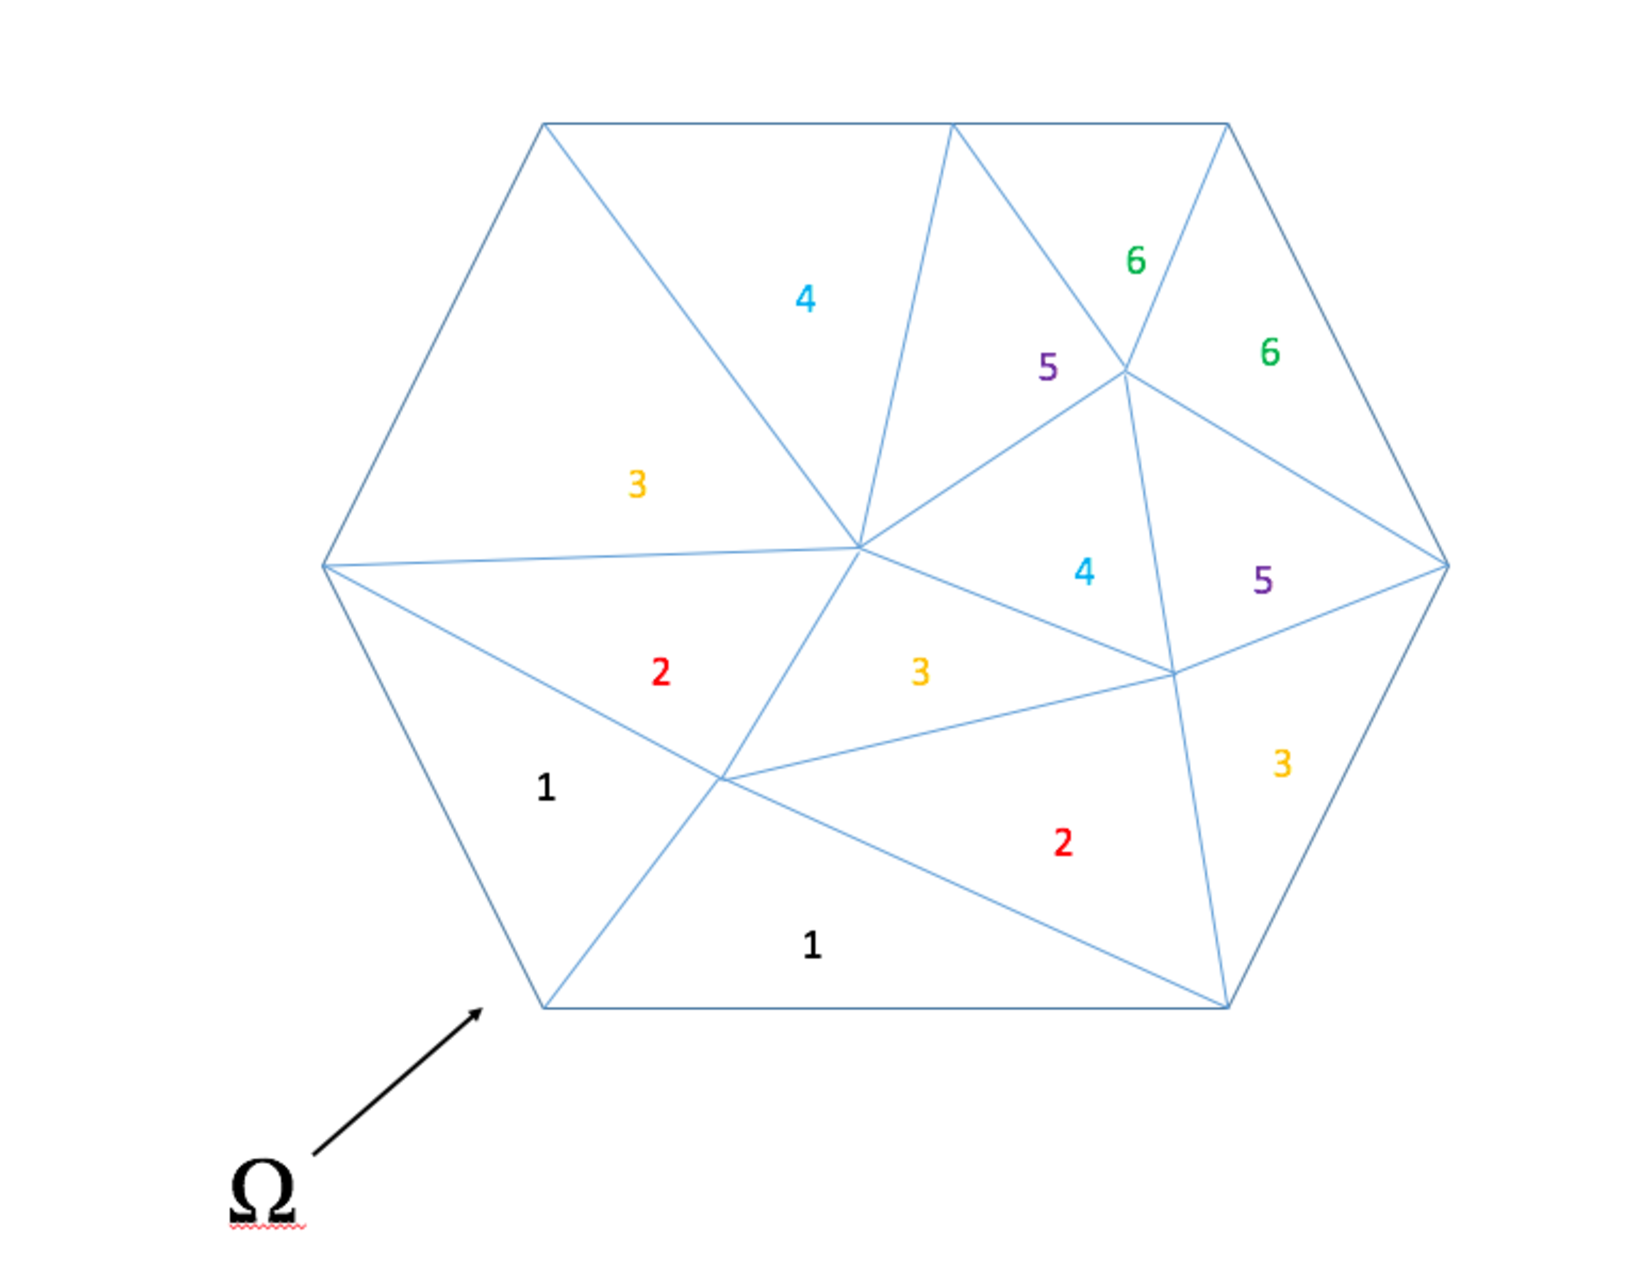
\includegraphics[scale = 0.15]{../figures/UnstructureMesh.pdf}
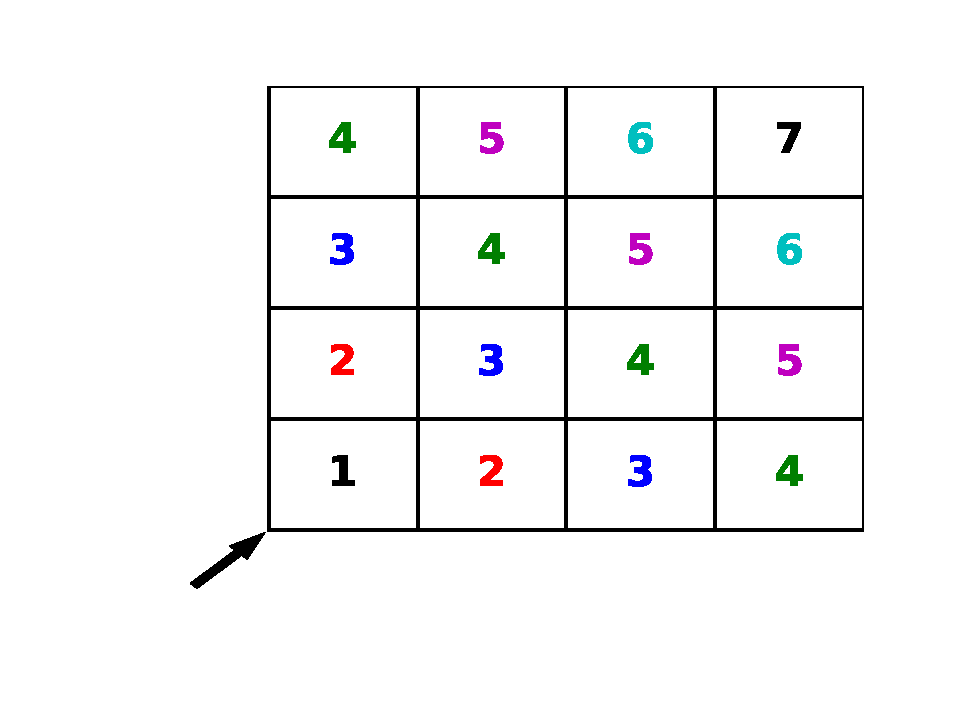
\includegraphics[scale = 0.15]{../figures/StructuredMesh.pdf}
\end{frame}

\begin{frame}[t]\frametitle{Parallel Transport Sweeps}

\begin{block}{A parallel sweep algorithm is defined by three properties:}
\begin{itemize}
\item partitioning: dividing the domain among available processors,
\item aggregation: grouping cells, directions, and energy groups into tasks,
\item scheduling: choosing which task to execute if more than one is available.
\end{itemize}
\end{block}
\end{frame}


\begin{frame}[t]\frametitle{KBA Algorithm}
\begin{block}{}
\begin{itemize}
\item KBA limits the number of processors in $z$ to one ($P_z$), solves one group at a time ($G=1$), and does not aggregate in angle or group ($A_g = A_m = 1$).
\item KBA primarily uses a "successive in angle, successive in quadrant" approach.
\item An octant pipelines its angular work, and once all directions are complete, the opposing octant pipelines them back.
\item This is then done for all remaining octant pairs.
\end{itemize}
\end{block}
\end{frame}

\begin{frame}[t]\frametitle{KBA Algorithm}
\begin{block}{}
\begin{itemize}
\item KBA utlilizes a "pipelining" or assembly line approach where new work is started before old work is fully completed.
\end{itemize}
\end{block}
\centering
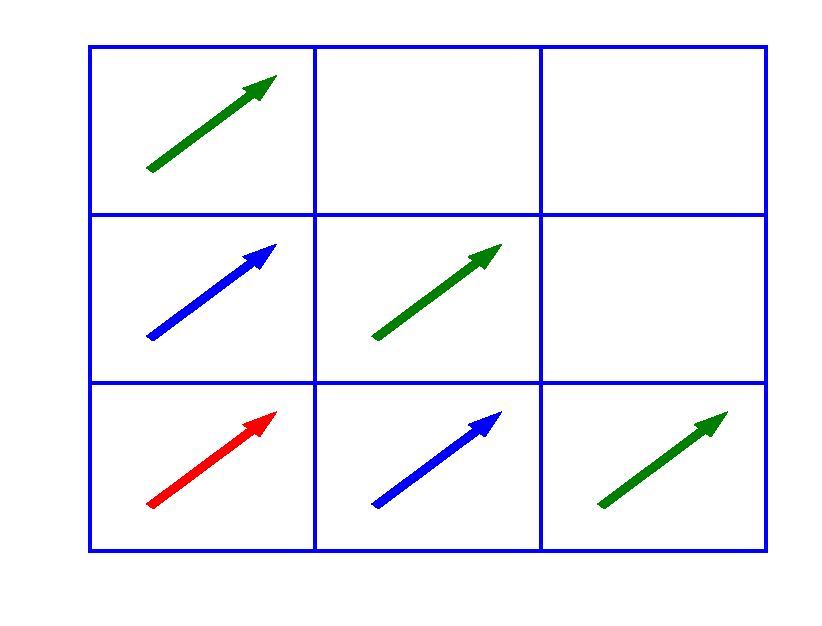
\includegraphics[scale=0.6,trim={0cm 1cm 0cm 0cm},clip]{../figures/pipeline_example.pdf}
\end{frame}

\begin{frame}[t]\frametitle{Sweeps in PDT}
\begin{block}{}
\begin{itemize}
\item PDT's extension of the KBA algorithm does not limit $P_z, A_m, G,$ or $A_g$.
\item PDT also launches all 8 octants (4 quadrants in 2D) simultaneously, rather than one octant-pair at a time.
\item Unlike KBA, PDT must schedule around conflicts that emerge between octants.
\end{itemize}
\end{block}
\end{frame}

\begin{frame}[t]\frametitle{Tie Breaking in PDT}

\begin{block}{If two or more tasks reach a processor at the same time, PDT employs a tie breaking strategy:}

\begin{enumerate}
	\item The task with the greater depth-of-graph remaining (simply, more work remaining) goes first.
	\item If the depth-of-graph remaining is tied, the task with $\Omega_x > 0$ wins.
	\item If multiple tasks have $\Omega_x > 0$, then the task with $\Omega_y > 0$ wins.
	\item If multiple tasks have $\Omega_y > 0$, then the task with $\Omega_z > 0$ wins.
\end{enumerate}
\end{block}
\end{frame}

\begin{frame}[t]\frametitle{Unstructured Meshing in PDT}
  \begin{block}{}
    \begin{itemize}
      \item PDT using unstructured meshes has been a priority since early 2014. 
      \item Unstructured meshes allow for simulation of a wider and more general variety of problems.
      \item Three unstructured mesh types are supported in PDT:
        \begin{itemize}
          \item Triangle (2D and 2D extruded triangular/prismatic meshes).
          \item Spiderweb (2D and 2D extruded prismatic meshes).
          \item Cubit/OpenFOAM (fully unstructured 3D meshes).
        \end{itemize}
    \end{itemize}
  \end{block}
\end{frame}

\begin{frame}[t]\frametitle{Unstructured Meshing in PDT}
\begin{block}{Partitioning for Unstructured Meshes}
\begin{itemize}
\item ``Cut lines'' in 2D (cut planes for 3D) are used to slice through the mesh in the $x$, $y$, and $z$ dimensions.
\item The cut planes form brick partitions, called subsets, that have unstructured meshes inside of them. 
\item The subsets are distributed amongst the processor domain.
\end{itemize}
\end{block}
\end{frame}

\begin{frame}[t]\frametitle{Partitioning Example}
\centering
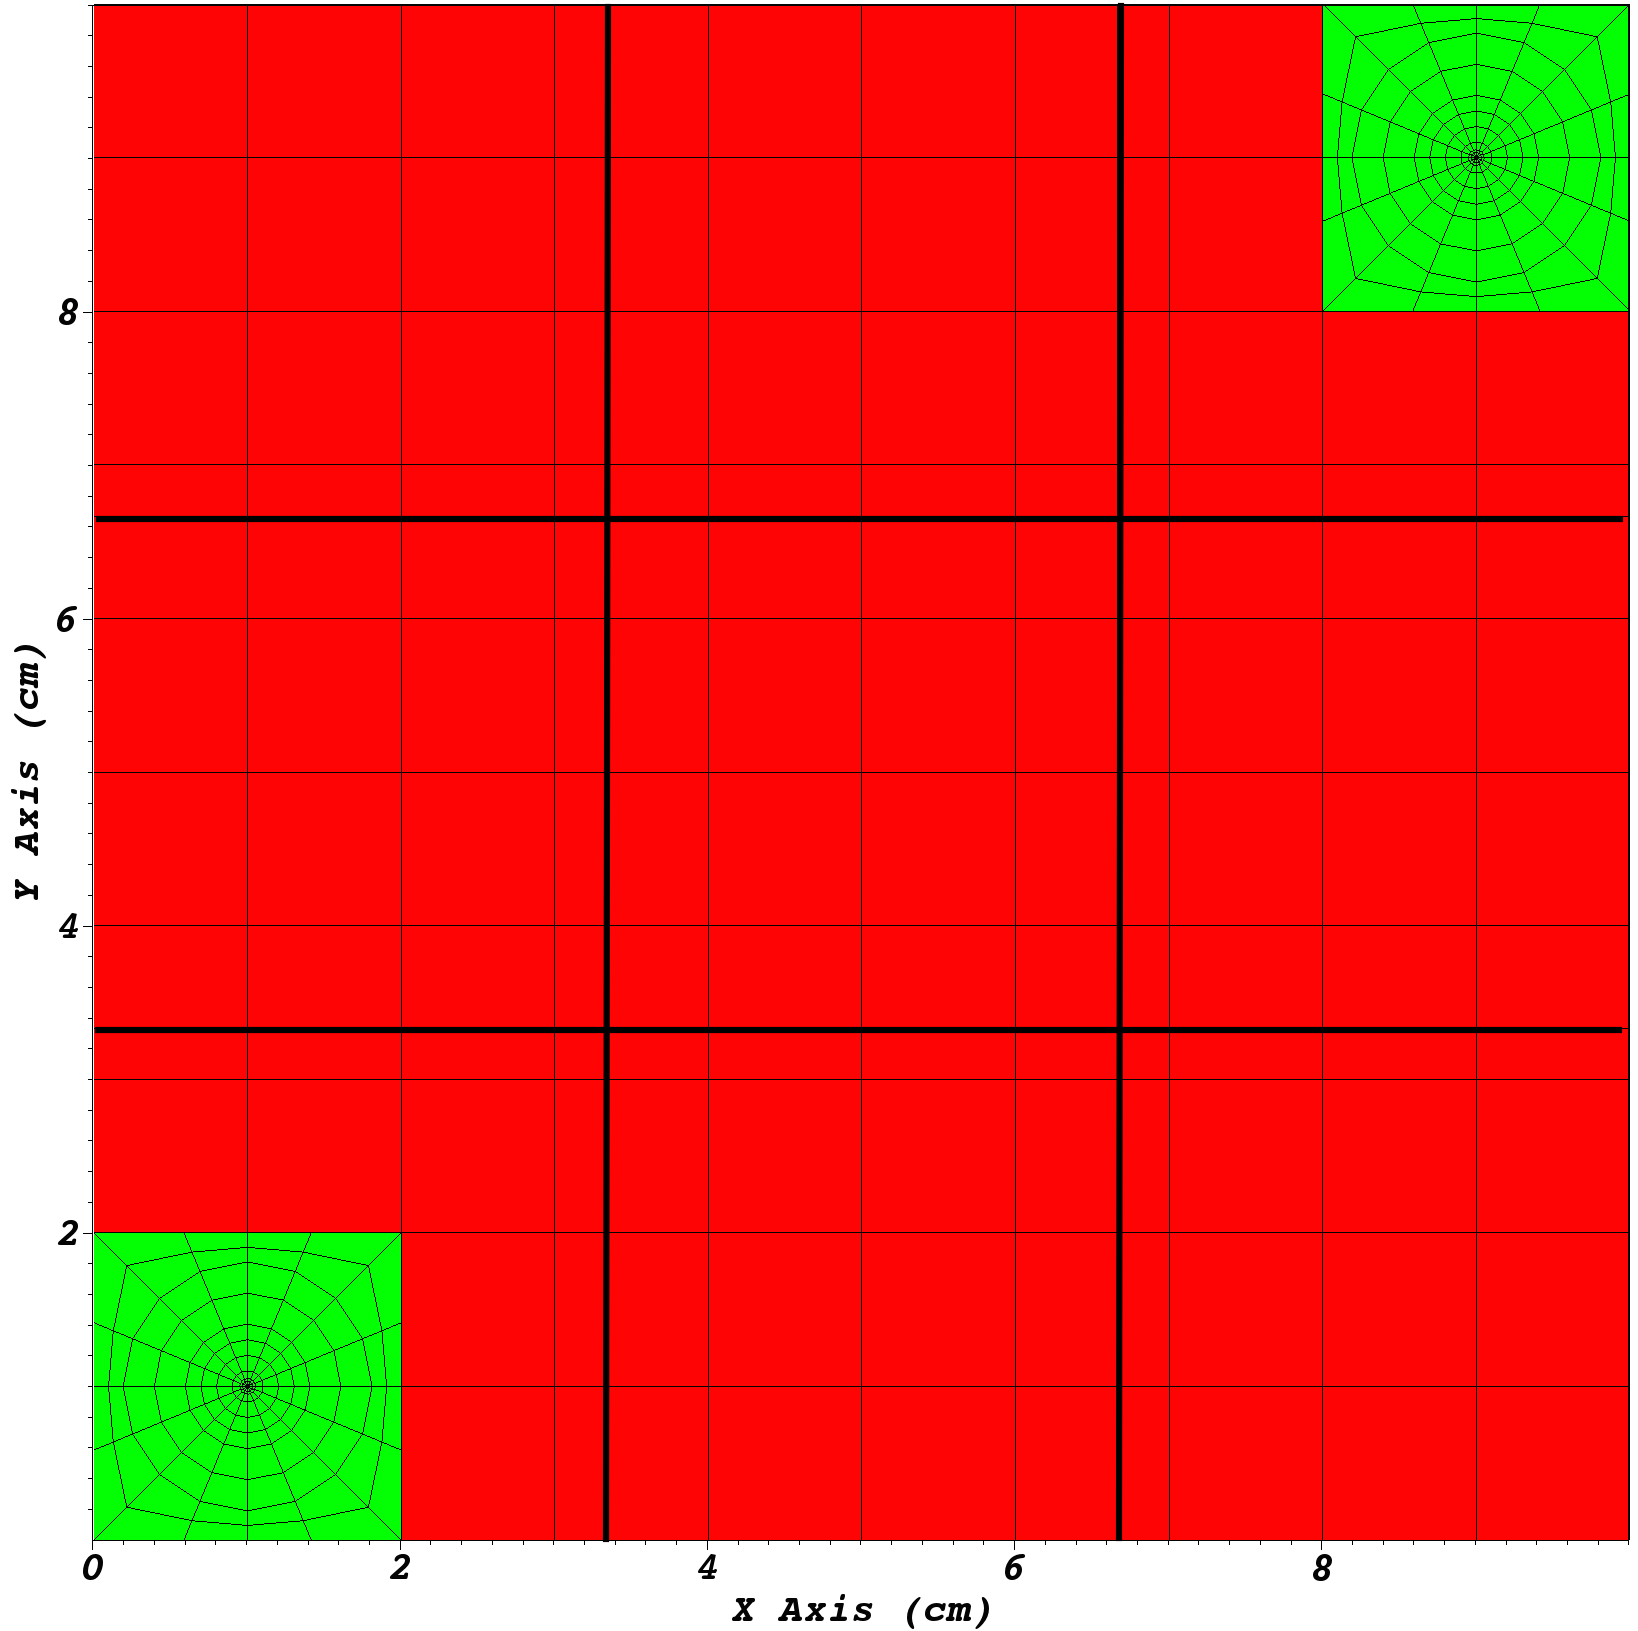
\includegraphics[scale=0.125]{../figures/ubp_3x3_regular.png}
\end{frame}


\section{Load Balancing}
\subsection{}

\begin{frame}[t]\frametitle{Load Balancing}
\begin{block}{Load Balance Metric}
  \begin{itemize}
    \item Max cells per subdomain divided by the average cells per subdomain:
      \begin{itemize}
        \item$f =\frac{\underset{ij}{\text{max}}(N_{ij})}{\frac{N_{tot}}{I\cdot J}}$
      \end{itemize}
    \item Column-wise metric: $f_I = \underset{i}{\text{max}}[\sum_{j} N_{ij}]/\frac{N_{tot}}{I}$
    \item Row-wise metric: $f_J = \underset{j}{\text{max}}[\sum_{i} N_{ij}]/\frac{N_{tot}}{J}$
  \end{itemize}		
  \tcr{Goal: minimize $f$ using locations of cut lines in X and Y}\\
    
  Subsequent improvement in algorithm: once dimension 1 has been balanced, balance dimension 2, then balance dimension 3 (\tcr{load balancing by dimension})
\end{block}
\end{frame}
\begin{frame}[t]\frametitle{Load Balancing Metrics}
\begin{equation}
f =\frac{\underset{ijk}{\text{max}}(N_{ijk})}{\frac{N_{tot}}{I\cdot J\cdot K}},
\label{metric_def}
\end{equation}
\begin{align}
f_{K} &= \underset{k}{\text{max}}[\sum_{i,j} N_{ijk}]/\frac{N_{tot}}{K}, \label{f_d1} \\
f_{I,k} &= \Big(\underset{i}{\text{max}}[\sum_{j} N_{ijk,k}]/\frac{N_{k}}{I}\Big), \label{f_d2}\\
f_{J,i,k} &= \Big( \underset{j}{\text{max}}[ N_{ijk,k,i}]/\frac{N_{k,i}}{J} \Big) . \label{f_j}
\end{align}
\end{frame}

\begin{frame}[t]\frametitle{Original Load Balancing Algorithm (2D Only)}
\begin{algorithm}[H]
\label{initial_algorithm}
\begin{algorithmic}

\WHILE{$f > \text{tol}_{\text{subset}}$}
  \IF {$f_I > \text{tol}_{\text{col}}$}
    \STATE Redistribute the X cut planes.
  \ENDIF
  \IF {$f_J > \text{tol}_{\text{row}}$}
  	\STATE Redistribute the Y cut planes.
  \ENDIF
\ENDWHILE
\end{algorithmic}
\end{algorithm}
\end{frame}

\begin{frame}[t]\frametitle{An example of redistributing cut lines}
\begin{figure}[H]
\centering
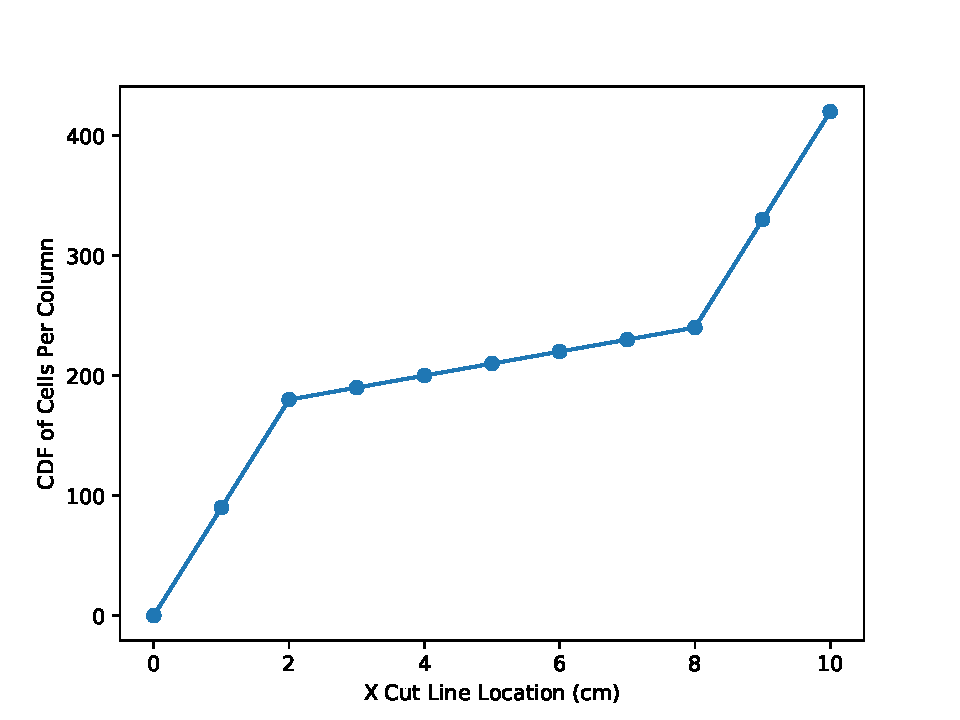
\includegraphics[scale=0.4]{../figures/spiderweb_redistribute_before_sparse.pdf}
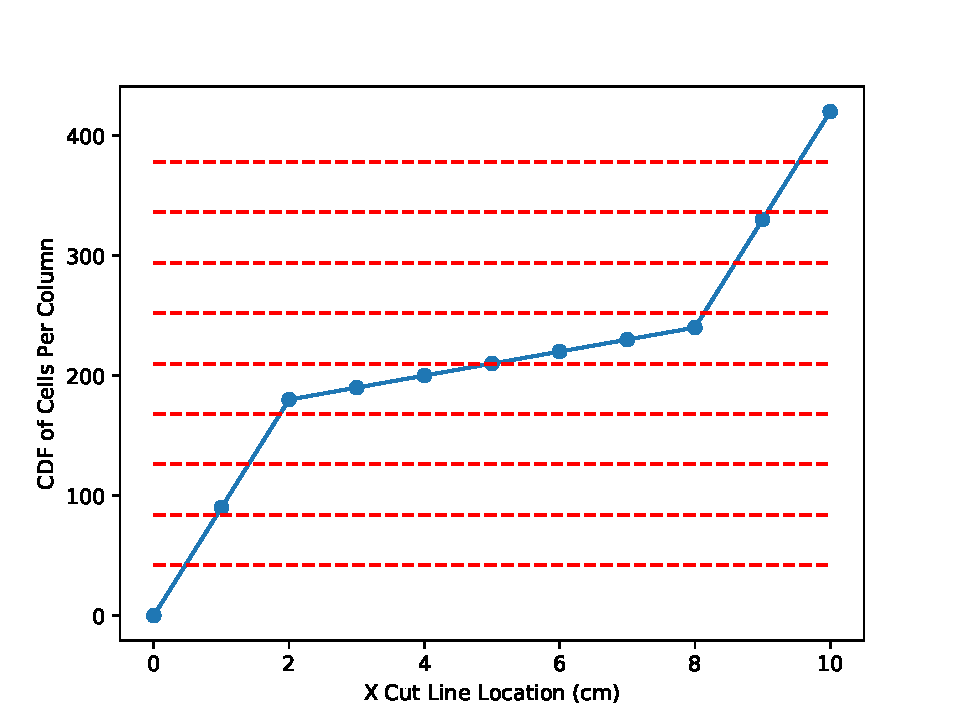
\includegraphics[scale=0.4]{../figures/spiderweb_redistribute_after_sparse.pdf}
\caption{The use of the CDF of cells per column to redistribute the cut planes in X.}
\label{redistribute}
\end{figure}
\end{frame}


\begin{frame}[t]\frametitle{No Load Balancing, f = 3.41}
\centering
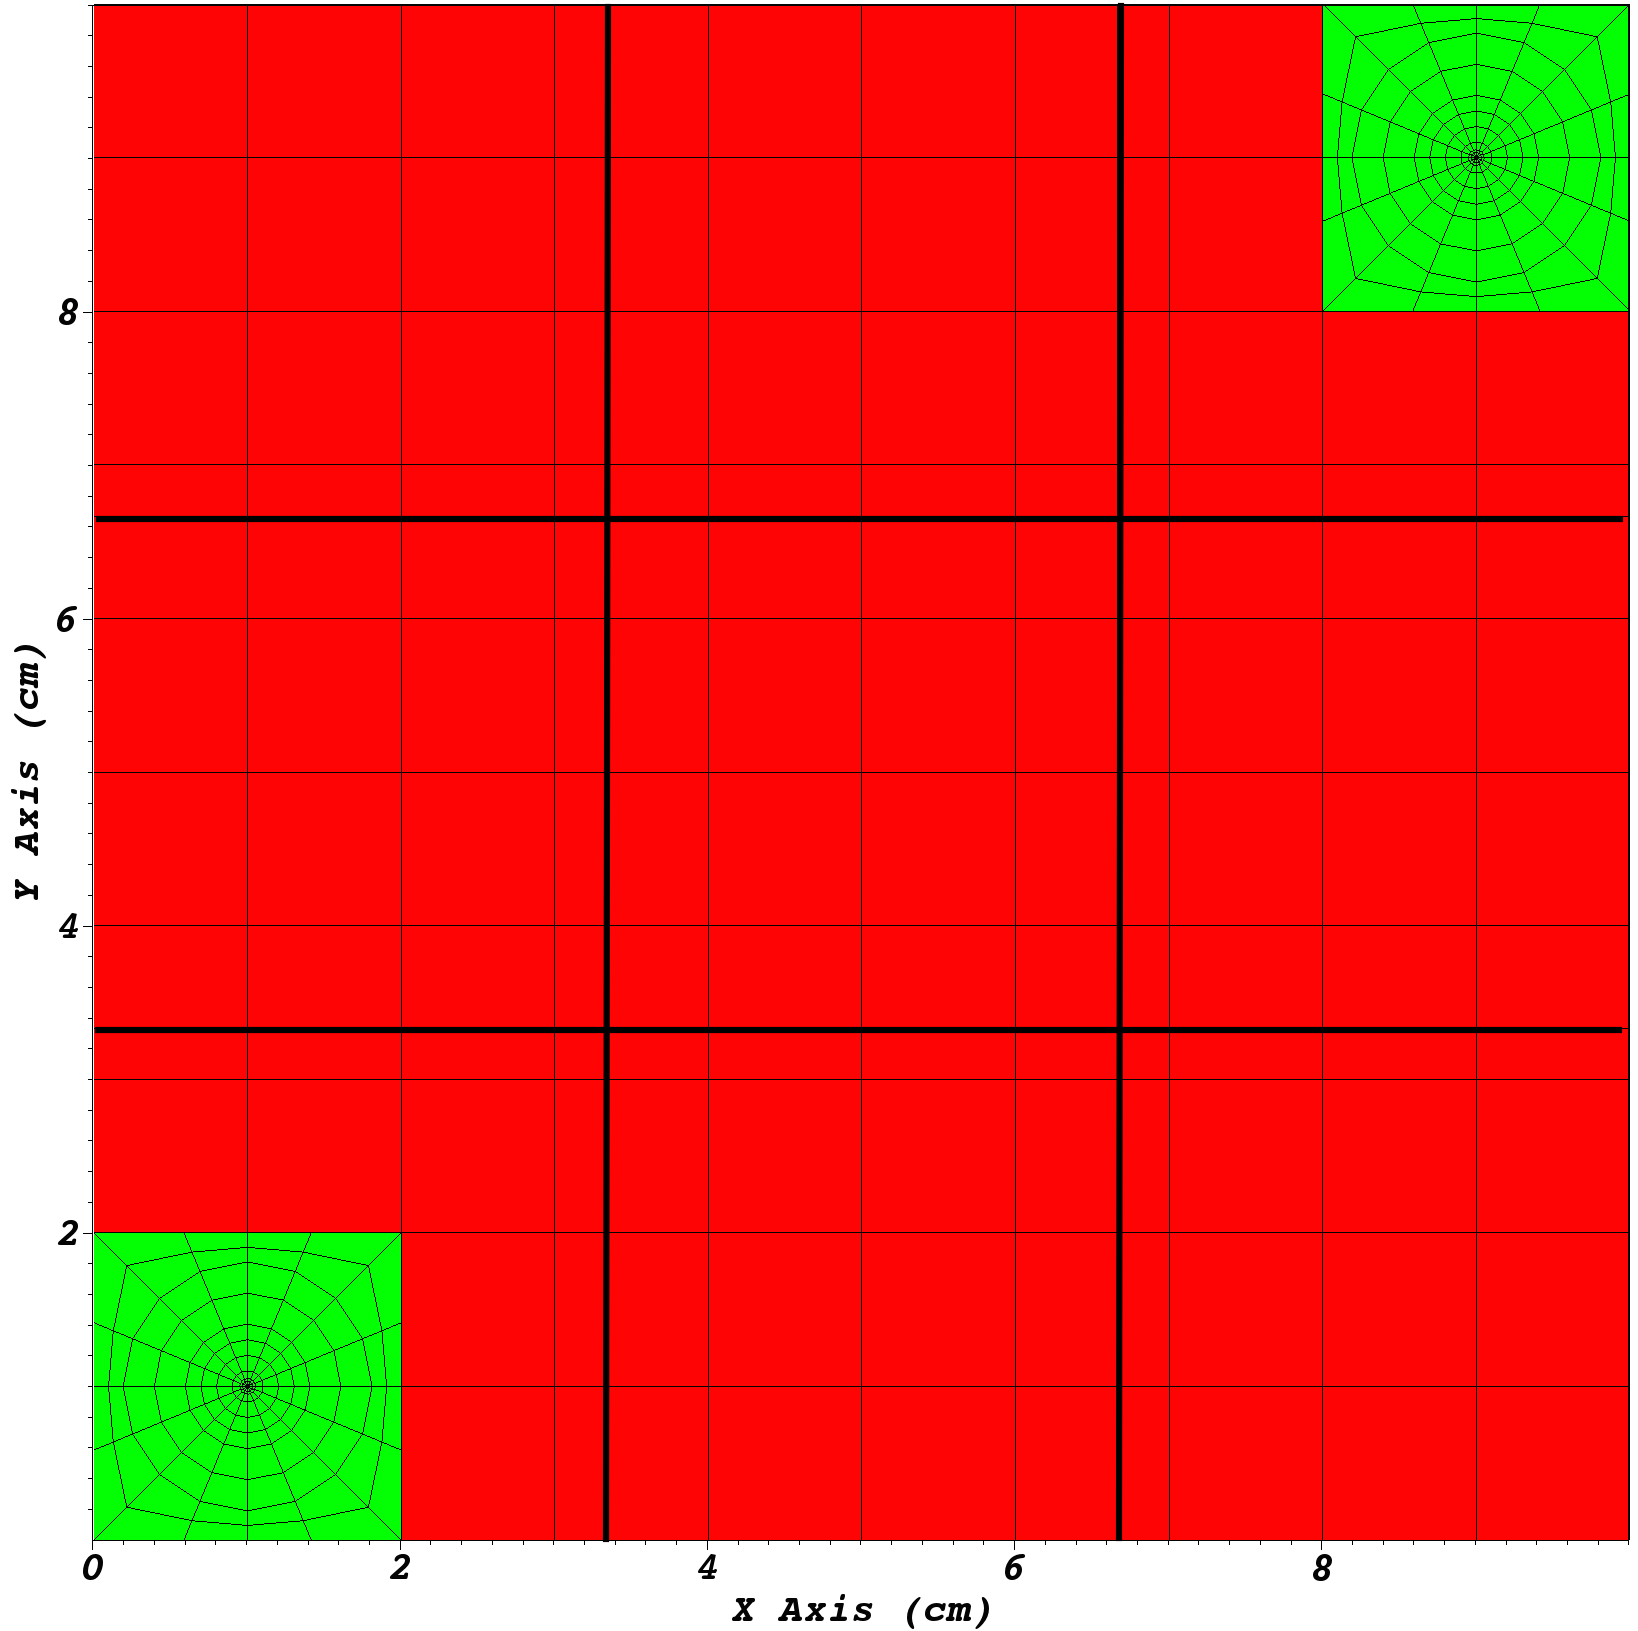
\includegraphics[scale=0.13]{../figures/ubp_3x3_regular.png}
\end{frame}

\begin{frame}[t]\frametitle{ 5 Load-Balancing Iterations, f = 2.58}
\centering
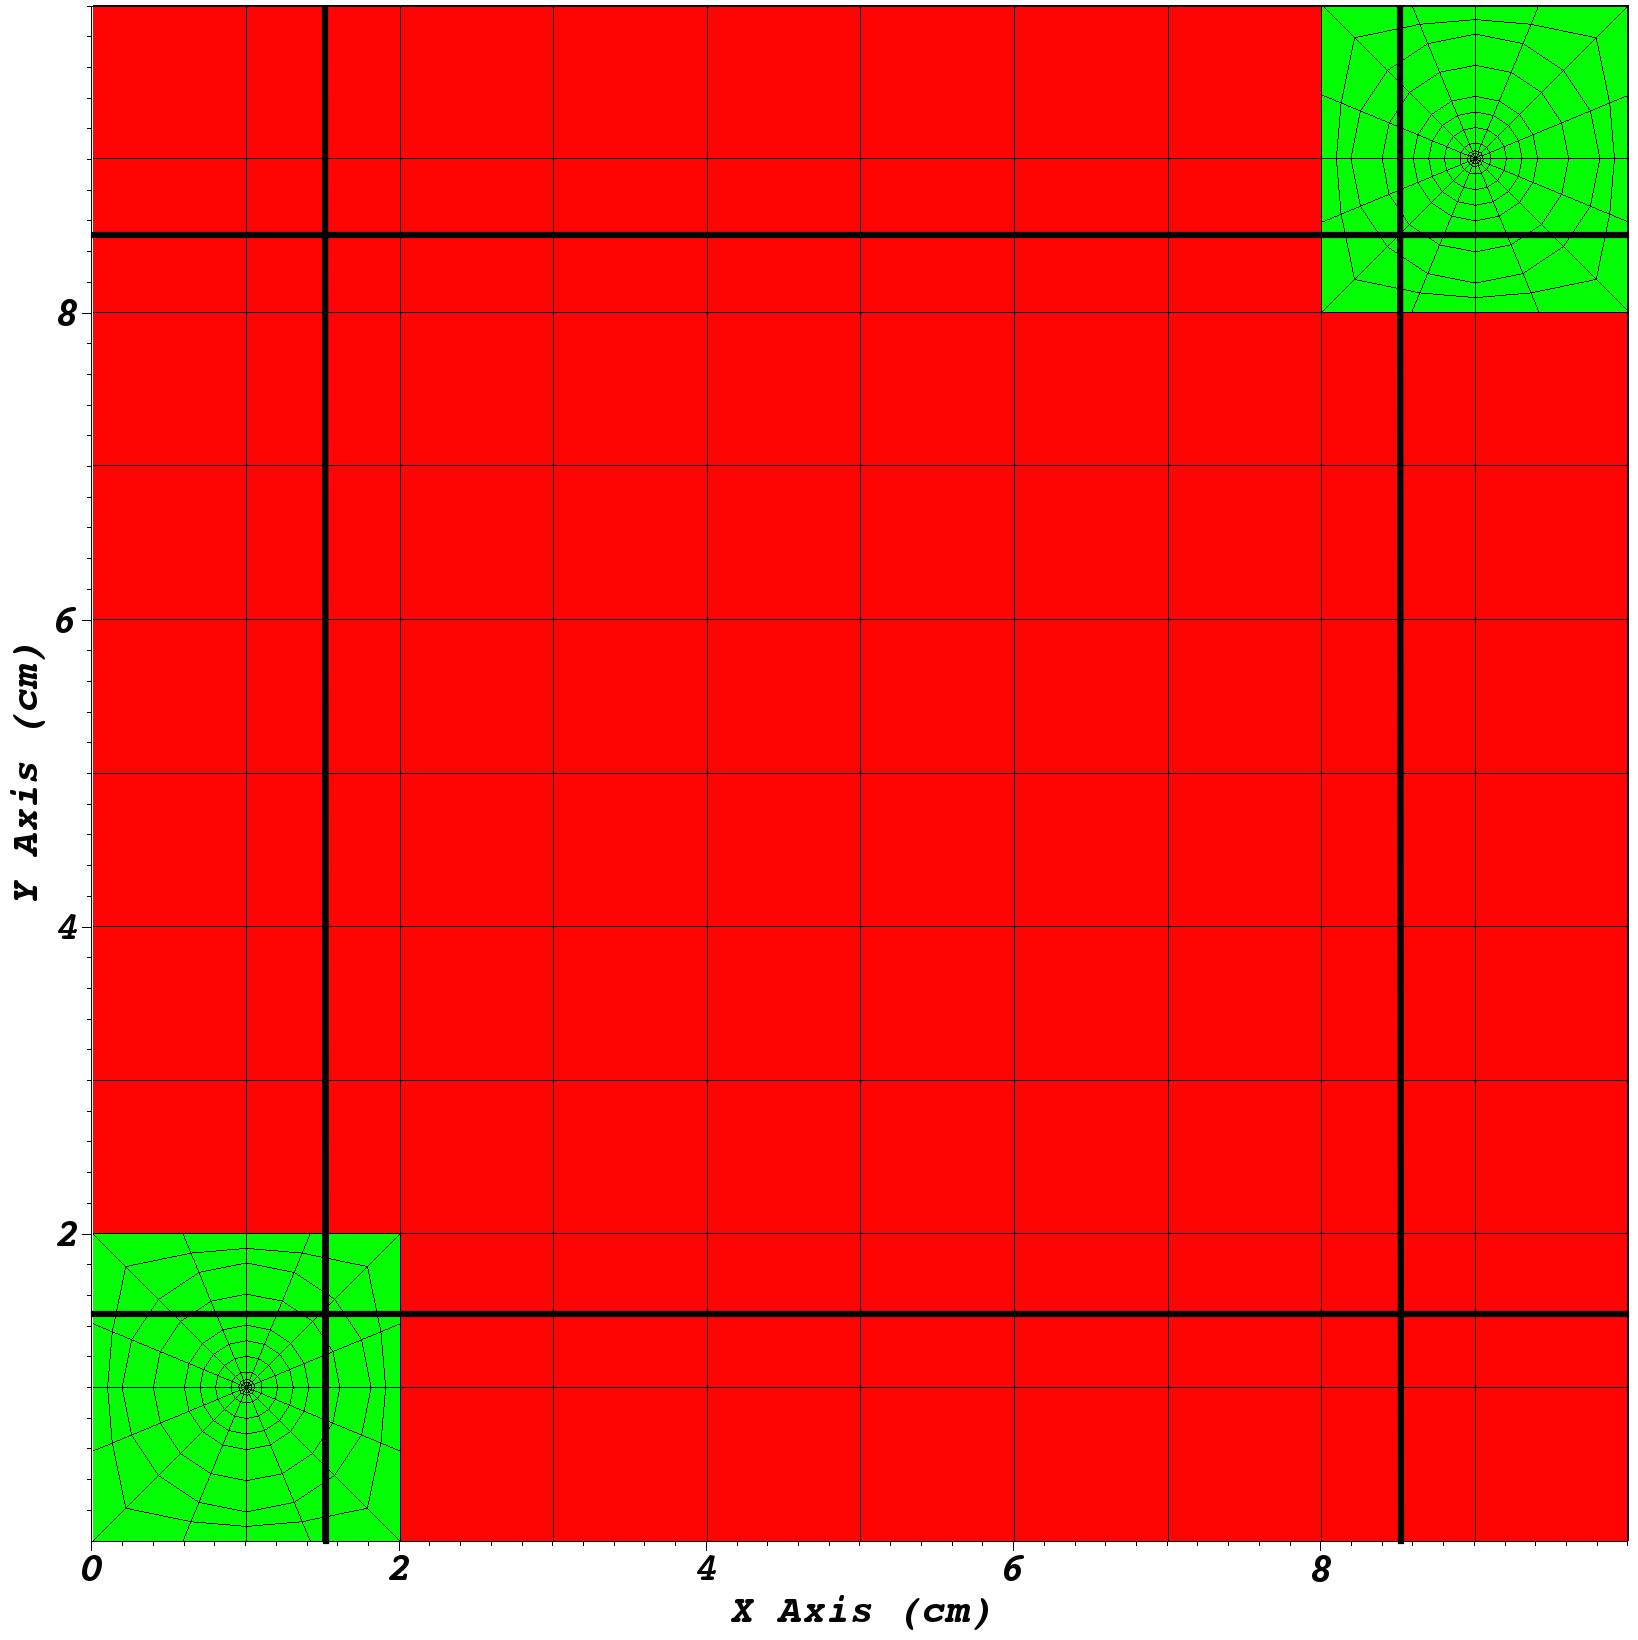
\includegraphics[scale=0.13]{../figures/ubp_3x3_lb.png}
\end{frame}

\begin{frame}[t]\frametitle{Theoretical Motivation for LBD}
  \begin{block}{}
  \begin{itemize}
    \item Consider simple 2D layout with $M$ unaligned subsets of high mesh density that each have $N$ cells.
    \item There are $M^2$ subsets, but only M have much work.
    \item Load Imbalance Factor $= \frac{N}{(MN+C)/M^2} \xrightarrow{N\to \infty} \frac{N}{N/M} = M$
  \end{itemize}
  \end{block}
  \begin{center}
    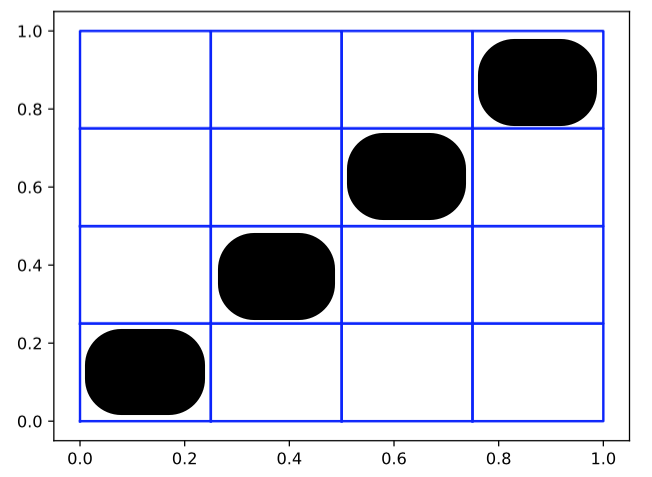
\includegraphics[scale=0.2]{../figures/theoretical_plot.png}
  \end{center}
\end{frame}

\begin{frame}[t]\frametitle{Load Balancing By Dimension Algorithm}
\begin{algorithm}[H]
\label{lbd}
\begin{algorithmic}

  \WHILE {$f_{K} > \text{tol}_{\text{K}}$}
    \STATE Redistribute the Z cut planes.
  \ENDWHILE  
  
  \FOR {$k$ in $K$}
    \WHILE {$f_{I,k} > \text{tol}_{\text{I}}$}
      \STATE Redistribute the X cut planes within each Z layer. 
    \ENDWHILE
  \ENDFOR
  
  \FOR{$k$ in $K$}
    \FOR{$i$ in $I$}
      \WHILE {$f_{J,i,k} > \text{tol}_{\text{J}}$ }
        \STATE Redistribute the Y cut planes within each column within each Z layer. 
      \ENDWHILE
    \ENDFOR
  \ENDFOR
  
  \STATE Calculate $f$.
\end{algorithmic}
\end{algorithm}
\end{frame}

\begin{frame}[t]\frametitle{Load Balancing By Dimension, f = 1.49}
\centering
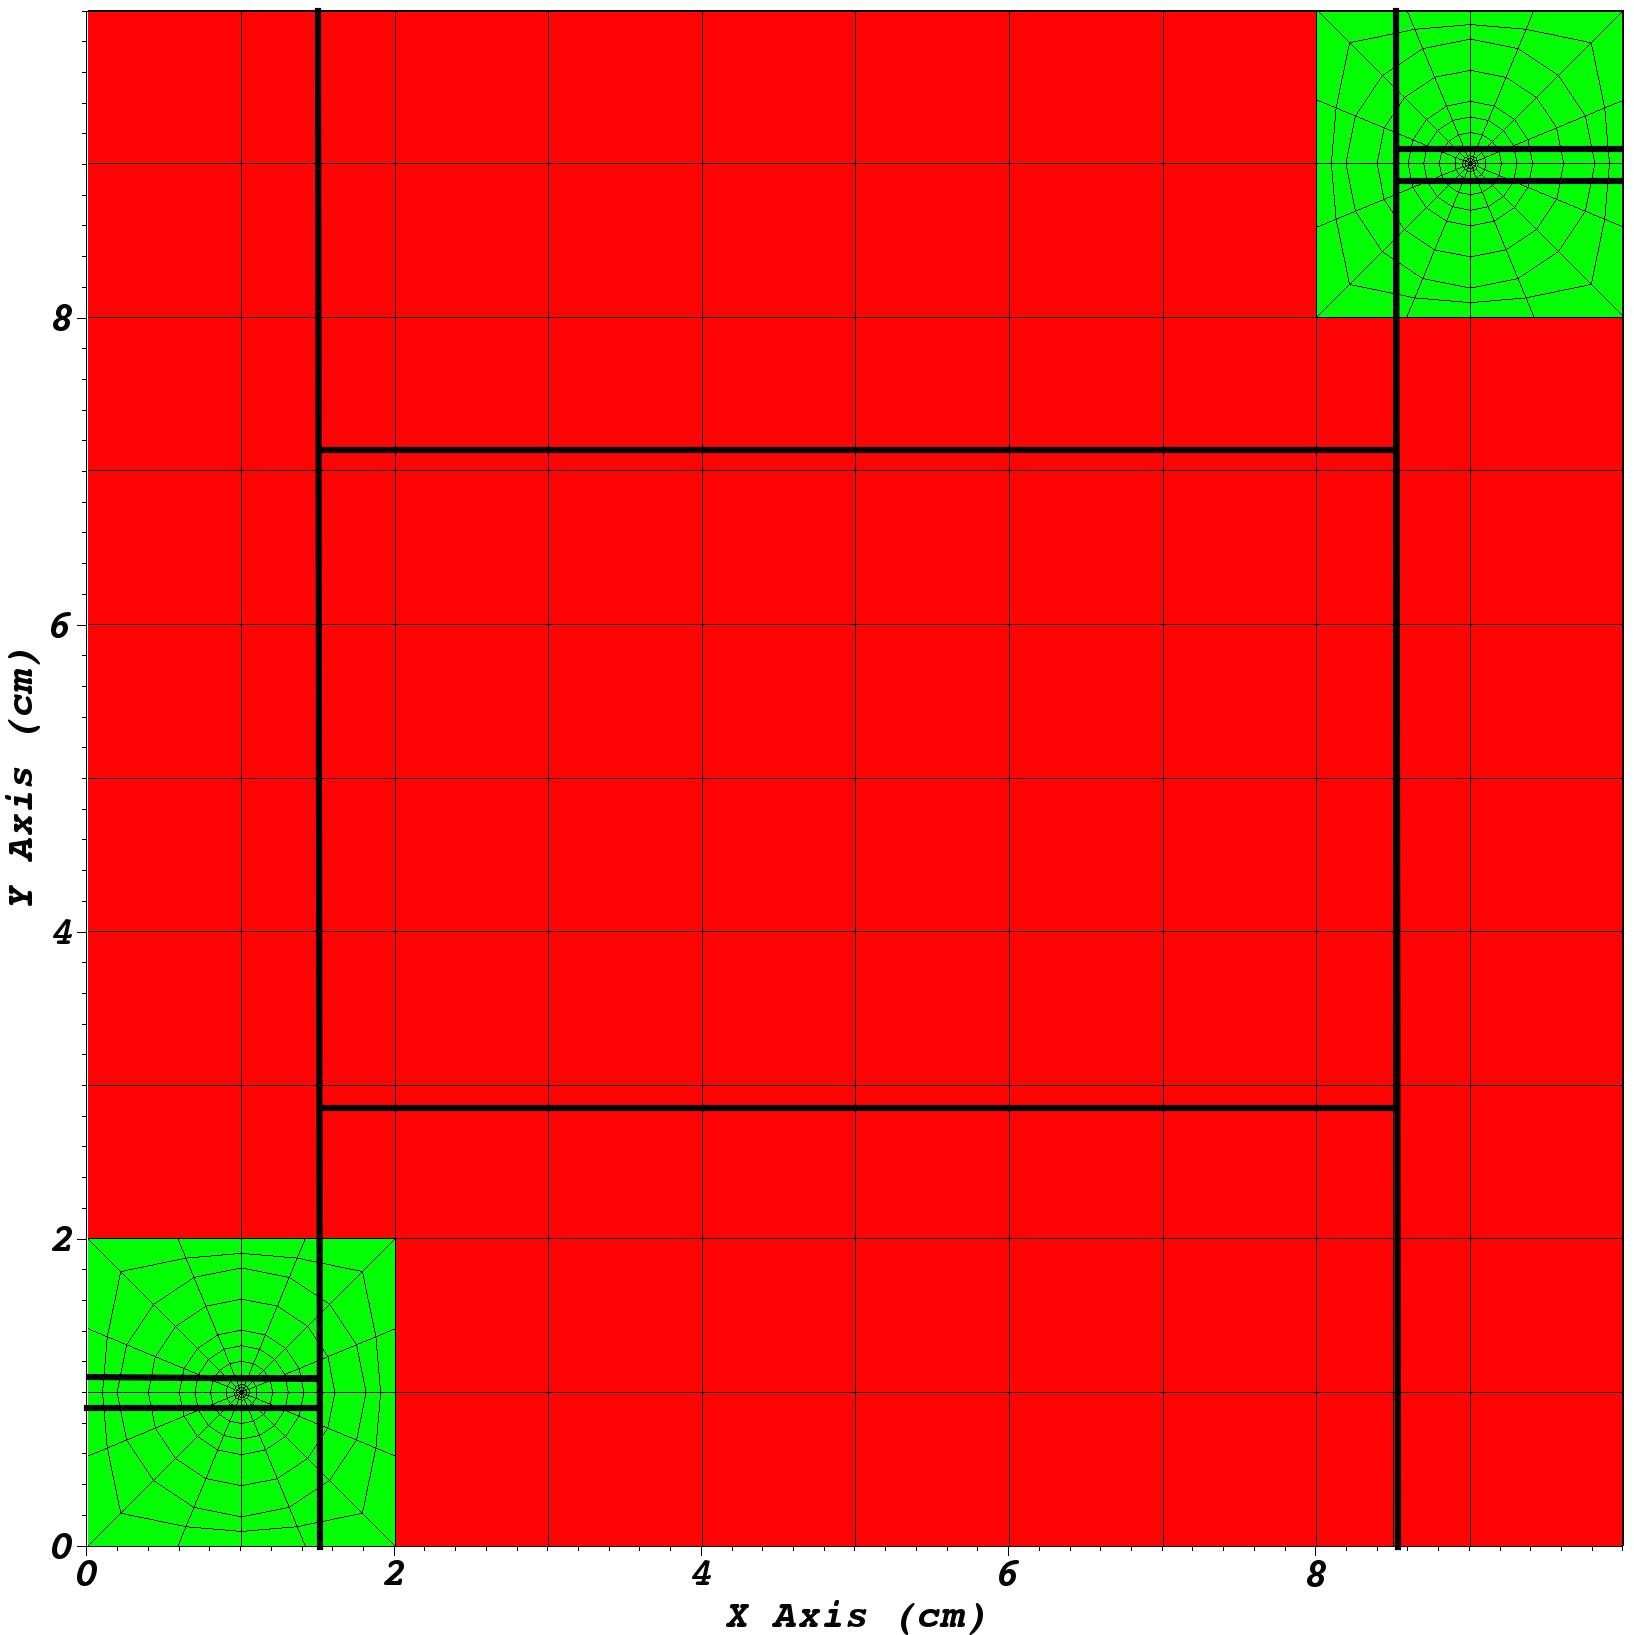
\includegraphics[scale=0.13]{../figures/ubp_3x3_lbd.png}
\end{frame}

\begin{frame}[t]\frametitle{3D Load Balancing By Dimension}
\centering
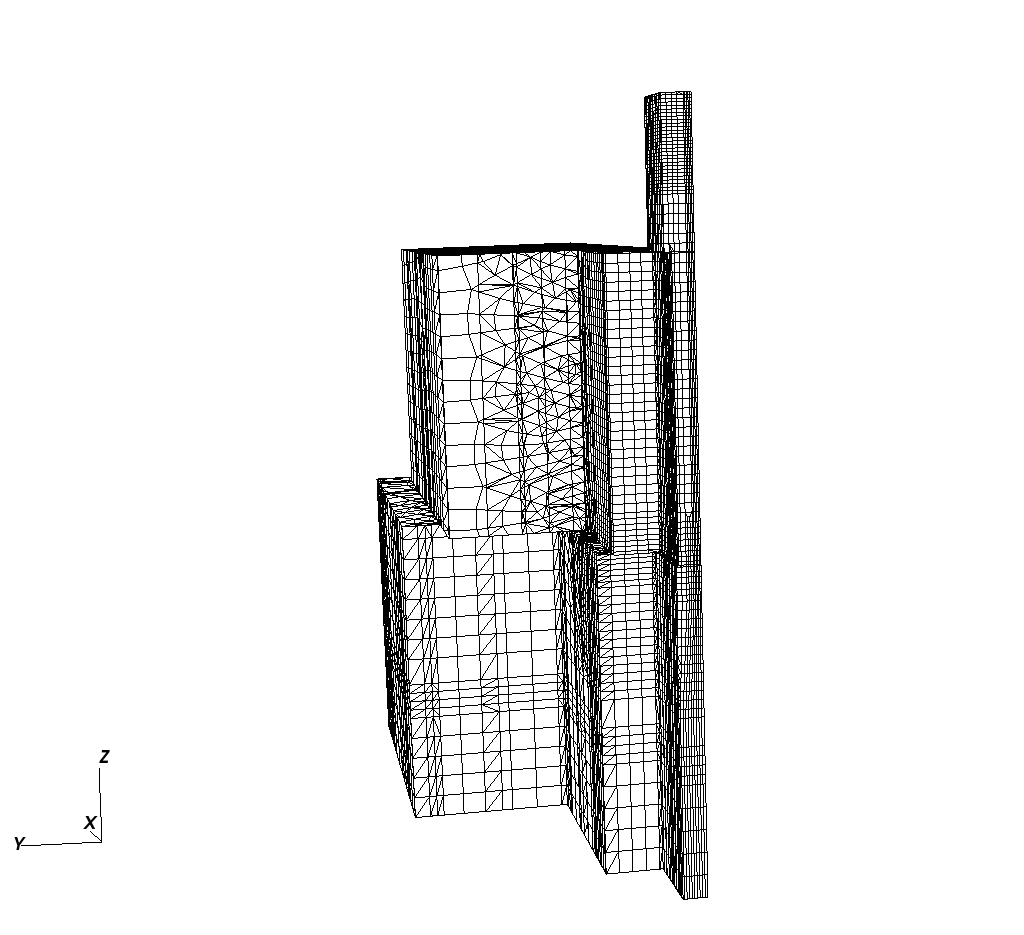
\includegraphics[trim={0cm 1cm 0cm 3cm},clip,scale=0.23]{../figures/im1_foam_448.png}
\end{frame}

\begin{frame}[t]\frametitle{Consequences of Load Balancing By Dimension}
  \begin{block}{}
  \begin{itemize}
    \item Perfect load balance in some cases will come at the cost of optimal sweeping.
    \item Time to solution is the most pertinent parameter, and if keeping a more optimal sweeping grid means a less balanced problem, then so be it.
    \item With imbalanced partitions it is harder to characterize the idle time, or the time where a processor has no work to do, and thus obtain an accurate stage count.
    \item A time-to-solution estimator must be built to more accurately predict sweep time.
  \end{itemize}
  \end{block}
\end{frame}

\begin{frame}[t]\frametitle{Sweep on Regular Grid with 3 Angle Sets}
    \centering
	\animategraphics[loop,controls,width=0.7\linewidth]{10}{../figures/sweeps_png/sweep_regular_20x20_as3_dog/sweep_regular_20x20_as3_dog_}{1}{48}
	%\href{run:figures/sweep_figs/sweeps_png/sweep_regular_20x20_as3_dog/animation.gif}{Animation.gif}
\end{frame}

\begin{frame}[t]\frametitle{Sweep on LBD Grid with 3 Angle Sets}
   \centering
	\animategraphics[loop,controls,width=0.7\linewidth]{10}{../figures/sweeps_png/sweep_random_20x20_as3_dog/sweep_random_20x20_as3_dog_}{1}{101}
	%\href{run:figures/sweep_figs/sweeps_png/sweep_random_20x20_as3_dog/animation.gif}{Animation.gif}
\end{frame}


\begin{frame}[t]\frametitle{Sweep on Worst Grid with 1 Angle Set}
    \centering
	\animategraphics[loop,controls,width=0.7\linewidth]{10}{../figures/sweeps_png/sweep_worst_20x20_as1_dog/sweep_worst_20x20_as1_dog_}{1}{230}
	%\href{run:figures/sweep_figs/sweeps_png/sweep_worst_20x20_as1_dog/animation.gif}{Animation.gif}
\end{frame}

%%%%%%%%%%%%%%%%%%%%%%%%%%%%%%%%%%%%%%%%%%%%%%%%%%%%%%%%%%%%%%%%%%%%%%%%%%%%%%%%%%%%%%%
%%%%%%%%%%%%%%%%%%%%%%%%%%%%%%%%%%%%%%%%%%%%%%%%%%%%%%%%%%%%%%%%%%%%%%%%%%%%%%%%%%%%%%%
%%%%%%%%%%%%%%%%%%%%%%%%%%%%%%%%%%%%%%%%%%%%%%%%%%%%%%%%%%%%%%%%%%%%%%%%%%%%%%%%%%%%%%%
\section{Time-To-Solution Estimator}
\subsection{}
%%%%%%%%%%%%%%%%%%%%%%%%%%%%%%%%%%%%%%%%%%%%%%%%%%%%%%%%%%%%%%%%%%%%%%%%%%%%%%%%%%%%%%%
%%%%%%%%%%%%%%%%%%%%%%%%%%%%%%%%%%%%%%%%%%%%%%%%%%%%%%%%%%%%%%%%%%%%%%%%%%%%%%%%%%%%%%%
%%%%%%%%%%%%%%%%%%%%%%%%%%%%%%%%%%%%%%%%%%%%%%%%%%%%%%%%%%%%%%%%%%%%%%%%%%%%%%%%%%%%%%%

\begin{frame}[t]\frametitle{Overview}
\begin{block}{}
\begin{itemize}
	\item We need to optimize the cut plane location not for balance, but for the best possible sweep time.
	\item We must build a time-to-solution estimator that calculates the time to solution for a given cut line partitioning and mesh cell density.
	\item The time to solution estimator will be fed into an optimizing function that minimizes the time to solution. The cut planes corresponding to the minimum time to solution are the optimal partitioning scheme.
\end{itemize}
\end{block}
\begin{block}{IMPORTANT}
The time-to-solution estimator is a graph-based method that uses graph algorithms that rely on an acyclic graph. The partitioning schemes used CANNOT induce cycles.
\end{block}
\end{frame}

\begin{frame}[t]\frametitle{Time To Solution Estimator}
\begin{block}{}
The time-to-solution estimator determines the time to sweep across a domain for a given partitioning scheme by:
\begin{enumerate}
	\item Building an adjacency matrix,
	\item Building Directed Acyclic Graphs (DAGs) from the adjacency matrix, one for each quadrant/octant,
	\item Weighting the edges of each graph based on the solve time and communication time of each subset to its neighbors,
  \item Adding and modifying graph weights based on how many anglesets are pipelined,
	\item Modifying the weights of each graph to operate on the universal timescale,
	\item Modifying the weights of each graph to reflect sweep conflicts between octants,
	\item Calculating the time to solution.
\end{enumerate}
\end{block}
\end{frame}

\begin{frame}[t]\frametitle{Building the Adjacency Matrix}
\begin{block}{}
\begin{itemize}
  \item The adjacency matrix provides the connectivity and ordering information necessary to build the Directed Acyclic Graphs (DAG) in the time-to-solution estimator.
\end{itemize}
\end{block}
\begin{figure}[H]
\centering
\begin{minipage}[c]{0.49\textwidth}
\centering
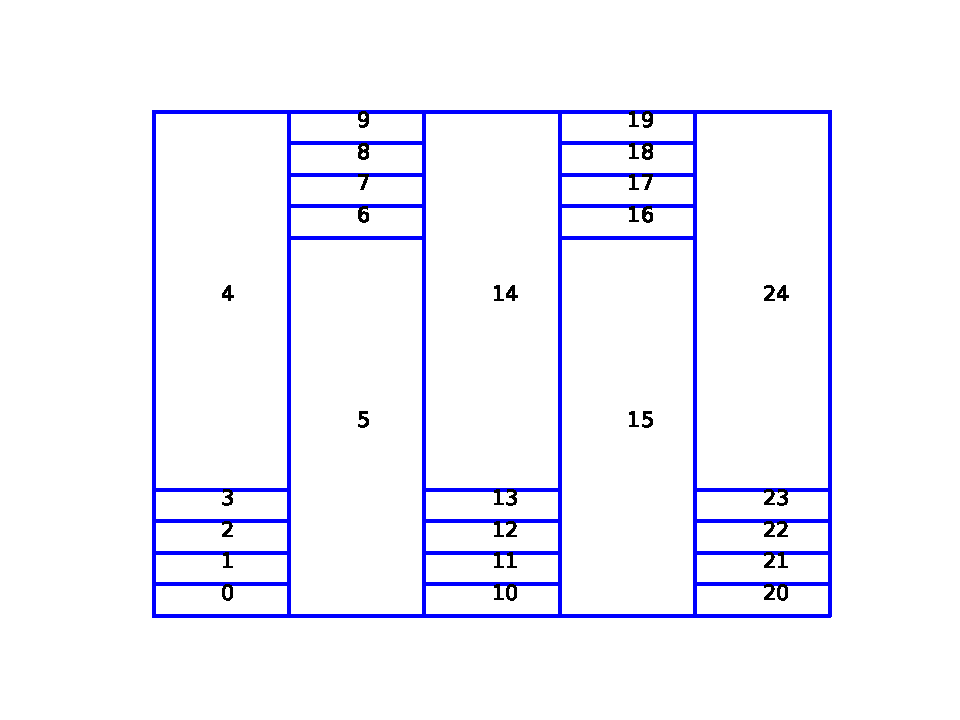
\includegraphics[scale=0.4]{../figures/boundaries_worst.pdf}
\end{minipage}
\begin{minipage}[c]{0.49\textwidth}
\centering
\scalebox{0.85}{
$\begin{pmatrix}
0&1&0&1&0&0&0&0&0\\
1&0&1&1&0&0&0&0&0\\
0&1&0&1&1&1&0&0&0\\
1&1&1&0&1&0&1&1&1\\
0&0&1&1&0&1&0&0&1\\
0&0&1&0&1&0&0&0&1\\
0&0&0&1&0&0&0&1&0\\
0&0&0&1&0&0&1&0&1\\
0&0&0&1&1&1&0&1&0\\
\end{pmatrix}$}
\end{minipage}
\caption{A 3x3 subset partitioning scheme and its corresponding adjacency matrix.}
\label{25basematrix}
\end{figure}
\end{frame}

\begin{frame}[t]\frametitle{Building the Directed Acyclic Graphs}
\begin{block}{}
\begin{itemize}
    \item Each quadrant/octant gets its own DAG.
    \item The opposing quadrant/octant pairs have opposing sweep orderings. 
    \item Python package \textbf{networkx} is used for all graph operations.
\end{itemize}
\end{block}
\centering
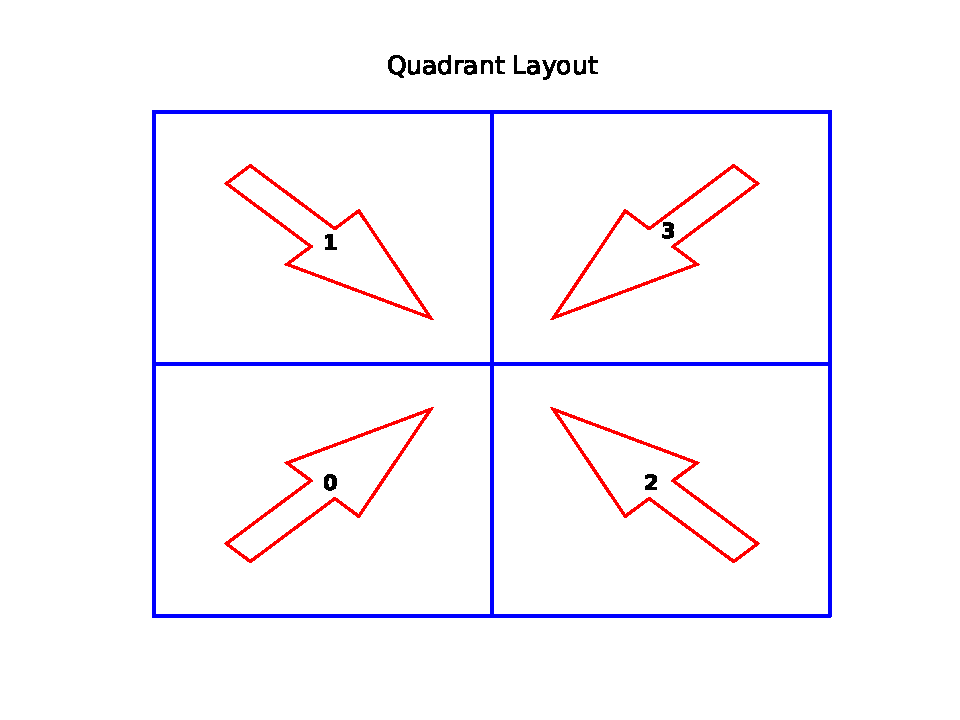
\includegraphics[scale=0.45]{../figures/quadrant_layout.pdf}
\end{frame}

\begin{frame}[t]\frametitle{The DAGs corresponding to the 3x3 partitioning scheme}
\begin{figure}
\centering
\begin{subfigure}[t]{0.49\textwidth}
\centering
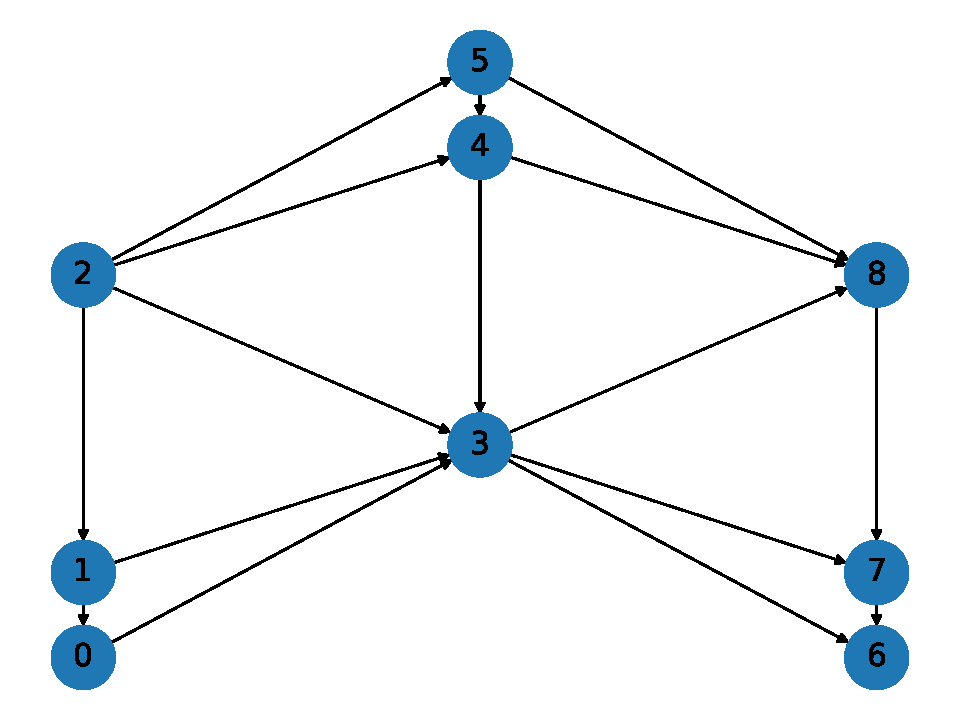
\includegraphics[scale=0.3]{../figures/9_graph1.pdf}
\end{subfigure}
\begin{subfigure}[t]{0.49\textwidth}
\centering
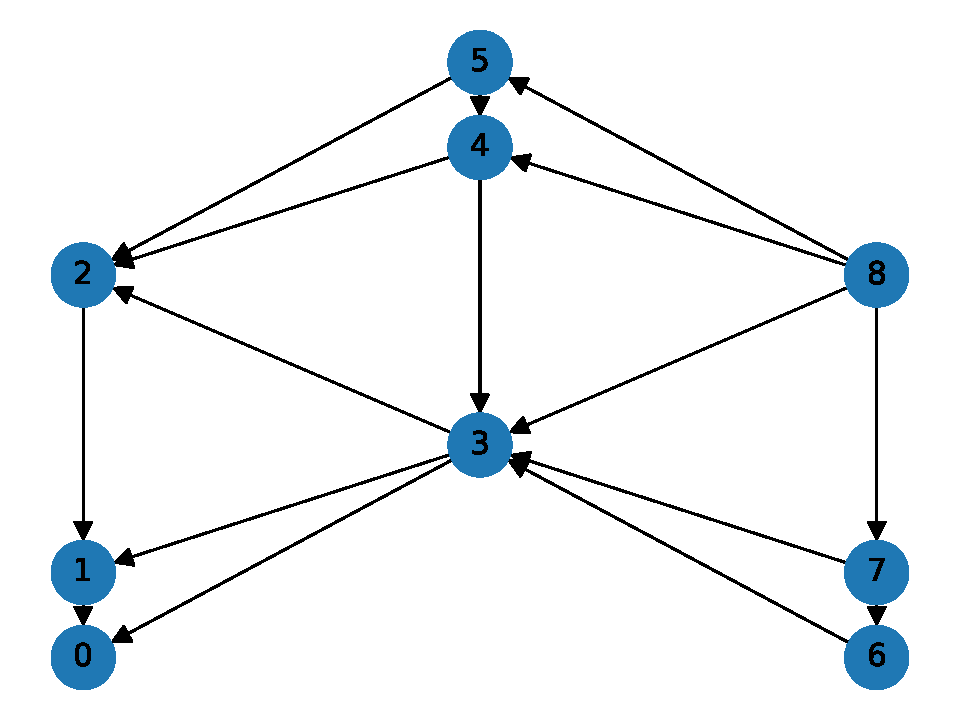
\includegraphics[scale=0.3]{../figures/9_graph3.pdf}
\end{subfigure}

\begin{subfigure}[t]{0.49\textwidth}
\centering
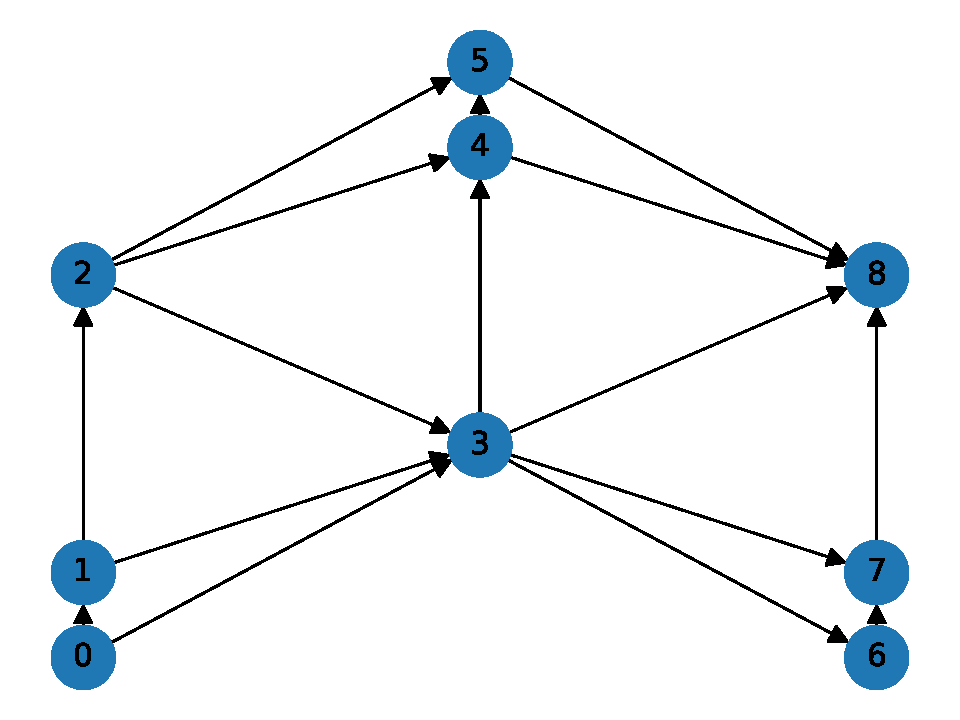
\includegraphics[scale=0.3]{../figures/9_graph0.pdf}
\end{subfigure}
\begin{subfigure}[t]{0.49\textwidth}
\centering
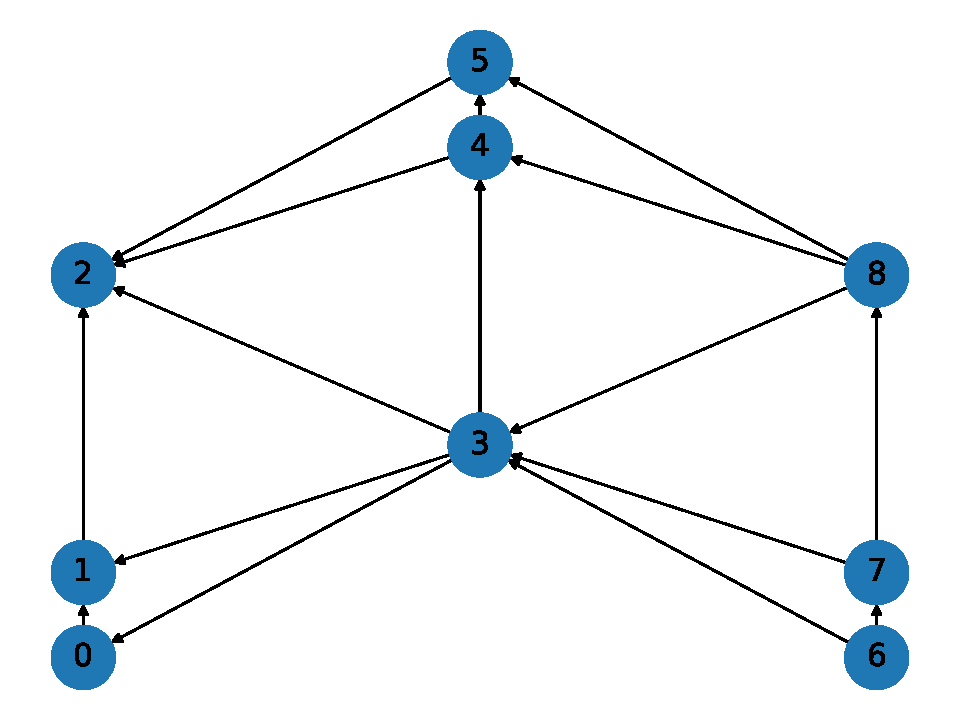
\includegraphics[scale=0.3]{../figures/9_graph2.pdf}
\end{subfigure}
\end{figure}
\end{frame}

\begin{frame}[t]\frametitle{Weighting the DAGs}
  \begin{block}{}
    Now that we have Directed Acyclic Graphs, we weight them with the help of PDT's performance model. 
  \end{block}
  \begin{block}{}
    Graph edge weight = time to solve cells in subset \& communicate boundary values to downwind subsets.
    \begin{align}
      \text{weight} = T_{wu} + N_c\cdot (T_c+ A_m\cdot(T_m + T_g)) + N_{b}\cdot A_m\cdot T_{\text{comm}} + T_{\text{latency}}
      \end{align}
    \begin{footnotesize}
    \begin{equation*}
    \begin{aligned}[c]
    N_c &= \text{number of cells}  \\
    A_m &= \text{Number of angles per task}  \\
    T_c &= \text{Time spent on cell-specific work}  \\
    T_{\text{comm}} &= \text{Comm time per double} \\ 
    \end{aligned}
    \begin{aligned}[c]
     N_b &=(\text{num boundary cells})\cdot \text{boundary unknowns per cell} \\
     T_m &= \text{Time spent on angle-specific work} \\
     T_g &= \text{Time spend on group-specific work} \\
     T_{wu} &= \text{Time to get into sweep operator} \\
     \end{aligned}
    \end{equation*}
    \end{footnotesize}
  \end{block}
\end{frame}

\begin{frame}[t]\frametitle{Weighting the DAGs}
  \begin{minipage}{0.49\textwidth}
    \centering
    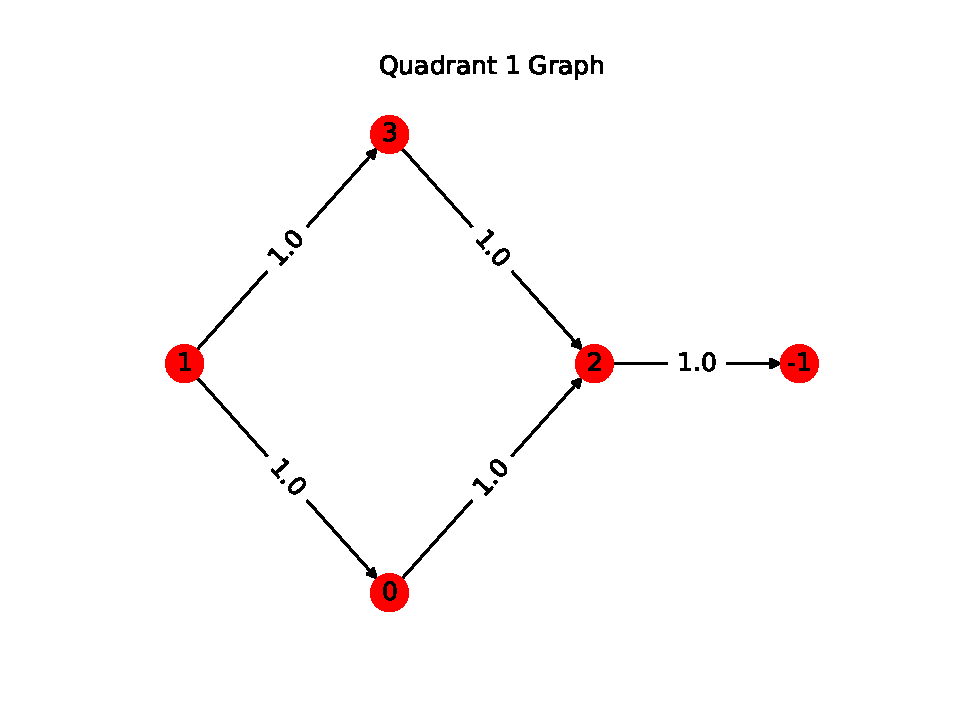
\includegraphics[scale=0.32]{../figures/q1_postweight.pdf}
  \end{minipage}
  \begin{minipage}{0.49\textwidth}
    \centering
    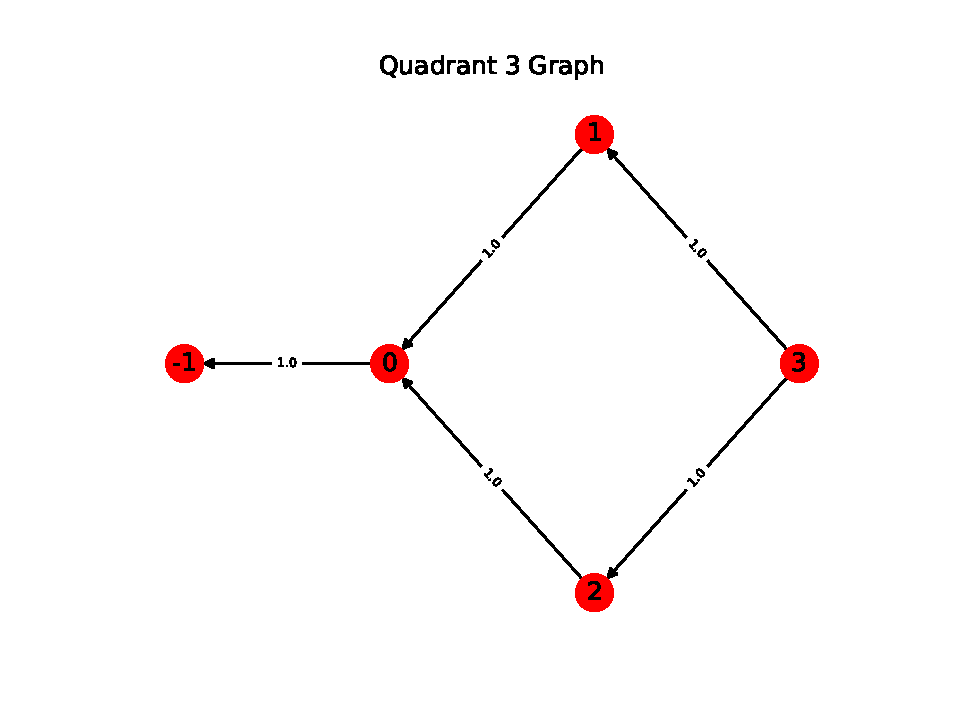
\includegraphics[scale=0.32]{../figures/q3_postweight.pdf}
  \end{minipage}
  \begin{minipage}{0.49\textwidth}
    \centering
    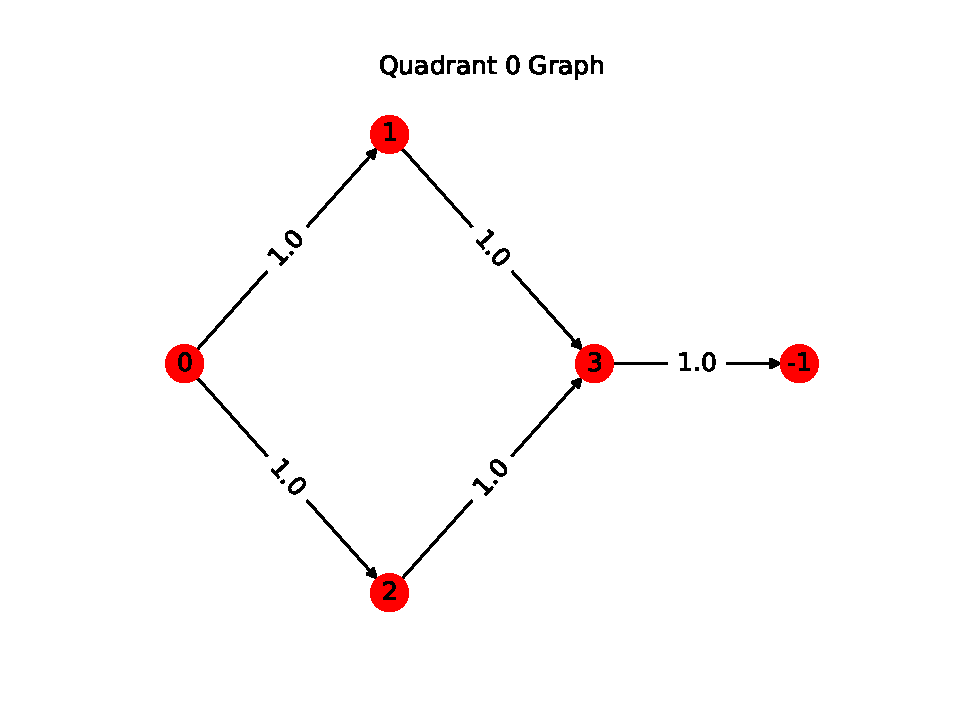
\includegraphics[scale=0.32]{../figures/q0_postweight.pdf}
  \end{minipage}
  \begin{minipage}{0.49\textwidth}
    \centering
    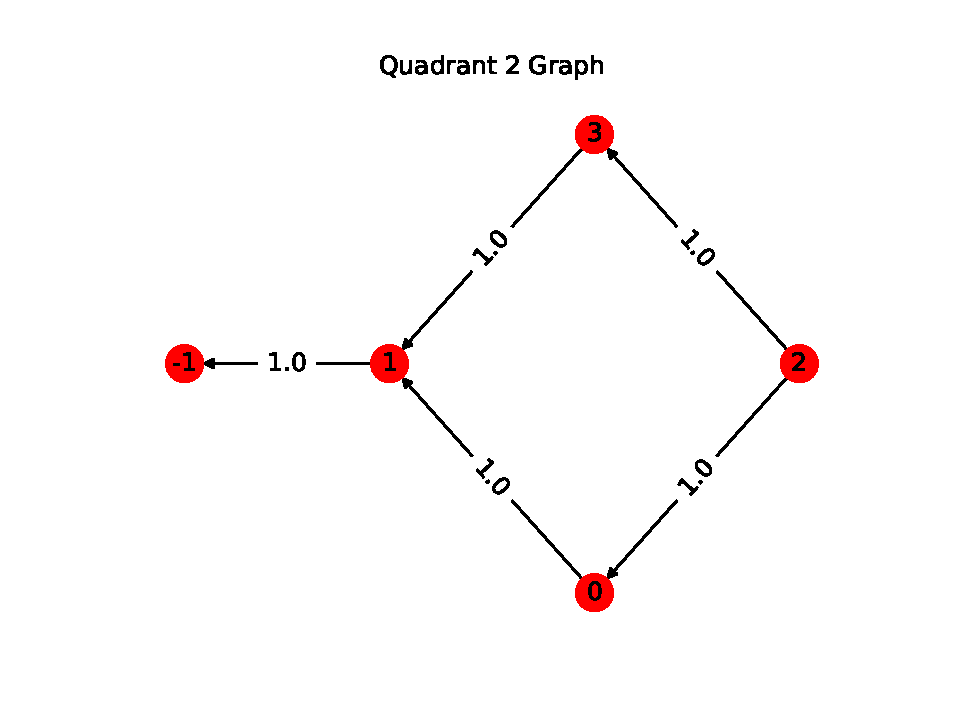
\includegraphics[scale=0.32]{../figures/q2_postweight.pdf}
  \end{minipage}
\end{frame}

\begin{frame}[t]\frametitle{Adding graphs for multiple anglesets}
\begin{figure}[H]
\begin{minipage}[c]{0.49\textwidth}
\centering
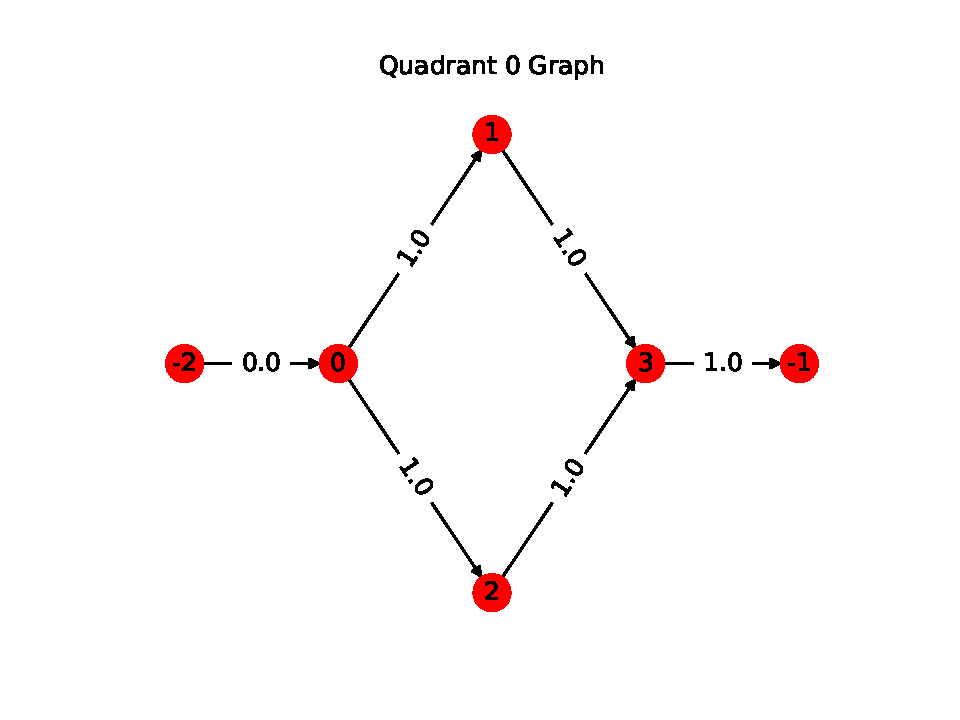
\includegraphics[scale=0.4]{../figures/q0_postpipeline.pdf}
\end{minipage}
\begin{minipage}[c]{0.49\textwidth}
\centering
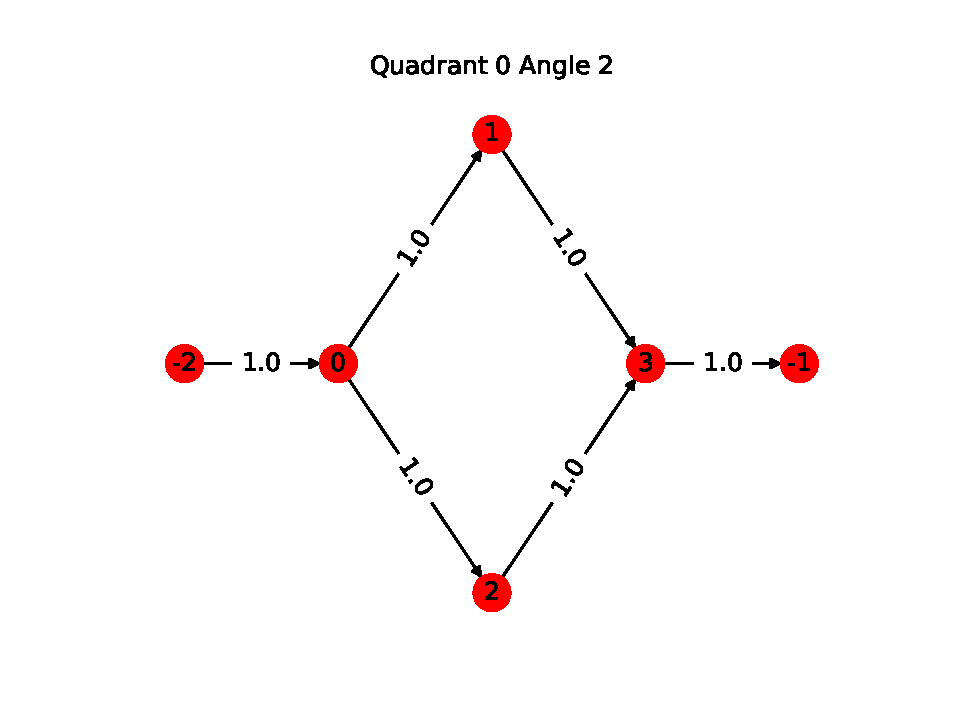
\includegraphics[scale=0.4]{../figures/q4_postpipeline.pdf}
\end{minipage}
\caption{The graphs for the first (left) and second (right) anglesets for quadrant 0.}
\label{angular_pipeline}
\end{figure}
\end{frame}

\begin{frame}[t]\frametitle{Modifying graph weights to reflect a universal timescale}
\begin{block}{}
  \begin{itemize}
    \item Once graphs are weighted for solve and communication time, we need to know when each node in each graph is ready to be solved.
    \item We calculate the sum of the longest weighted path to each node, and set all incoming edges of each node to this value.
    \item The incoming edges to each node now represent the time each node is ready to solve.
    \item The DAGs have now become Task Dependence Graphs (TDGs).
  \end{itemize}
\end{block}
\begin{figure}[H]
  \begin{minipage}[c]{0.49\textwidth}
    \centering
    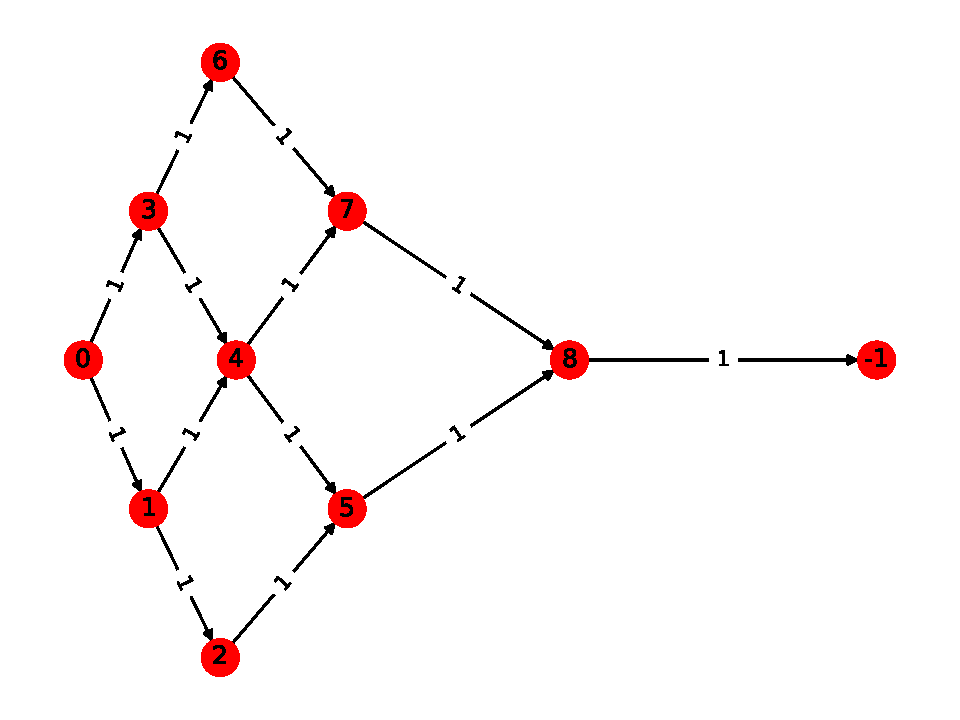
\includegraphics[scale=0.35]{../figures/G_pre_universal.pdf}
  \end{minipage}
  \begin{minipage}[c]{0.49\textwidth}
    \centering
    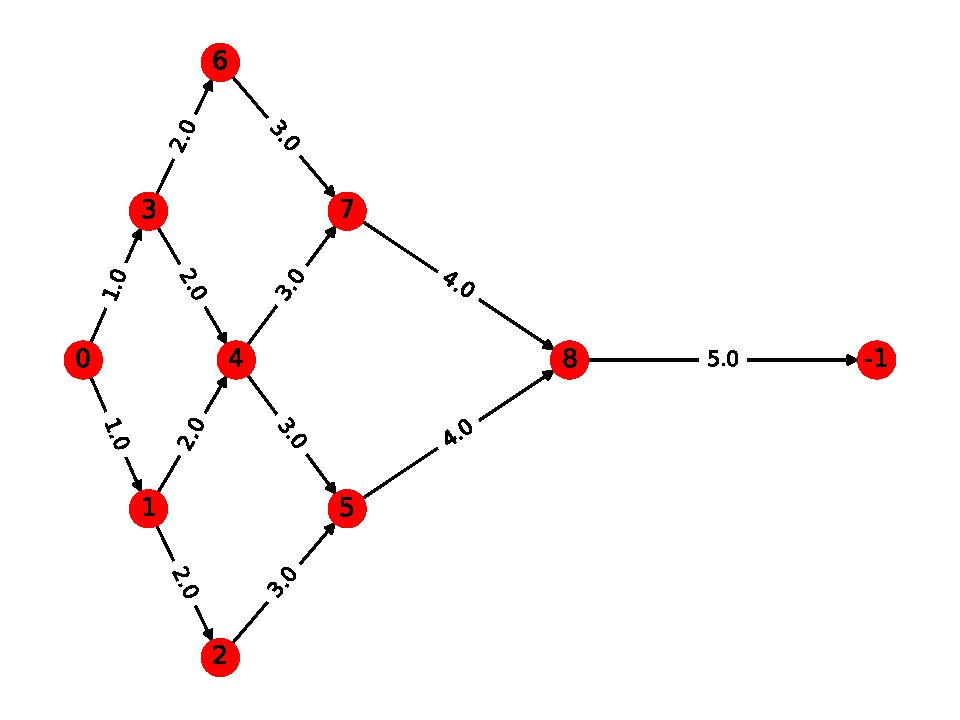
\includegraphics[scale=0.35]{../figures/G_universal.pdf}
  \end{minipage}
  \caption{A TDG before (left) and after (right) universal edge weighting is applied.}
   \label{universal}
\end{figure}
\end{frame}

\begin{frame}[t]\frametitle{Conflict Detection and Resolution}
  \begin{block}{}
    Best summarized as a ``marching'' process. 
    \begin{enumerate}
      \item Starting at time $t=0$, find the nodes that are ready to solve or already solving across all graphs.
      \item If at that time, multiple graphs are solving the same node, they are in conflict.
      \item The graph that ``wins'' the conflict does not have its weights modified, while the graph(s) that lose the conflict modify their downstream weights according to how long they are delayed.
      \item Update $t$ to the next interaction across all graphs.
      \item Repeat steps 2, 3, and 4 until all graphs are finished sweeping.
    \end{enumerate}
  \end{block}
\end{frame}

\begin{frame}[t]\frametitle{First Come First Serve Conflict Resolution}
\begin{block}{}
\begin{itemize}
	\item The first octant to arrive to a node will begin solving it, and the remaining octants will incur a delay (if applicable).
	\item The delay is reflected in each remaining TDG by adding the corresponding delay as a weight to the applicable edge and applicable downstream edges.
  \item If two octants arrive to a node at the same time, the octant with the greater remaining depth-of-graph and priority octant wins the tie.
\end{itemize}
\end{block}
\end{frame}

\begin{frame}[t]\frametitle{2D Verification}
\vspace{-0.3cm}
  \begin{block}{}
    \begin{itemize}
      \item A verification study was run to verify the time-to-solution estimator for 2D partitioning schemes with perfectly balanced partitions. 
      \item Verified against a code written by Dr. Ragusa that uses depth-of-graph with an octant-priority tiebreaker conflict resolution in two dimensions. 
    \end{itemize}
  \end{block}
  \begin{block}{Problems}
  \begin{small}
    \begin{enumerate}
      \item 2x2 to 10x10 subsets in x and y with regular partitions and 1 to 6 angles per quadrant.
	    \item 2x2 to 10x10 subsets in x and y with ``mildly random'' partitions and 1 to 6 angles per quadrant.
	    \item  2x2 to 10x10 subsets in x and y with ``random'' partitions and 1 to 6 angles per quadrant.
	    \item  2x2 to 10x10 subsets in x and y with probable worst-case partitions and 1 to 6 angles per quadrant.
    \end{enumerate}
    \end{small}
  \end{block}
\end{frame}

\begin{frame}[t]\frametitle{Regular Partitions}
  \vspace{-.35cm}
   \begin{minipage}{0.49\textwidth}
    \centering
    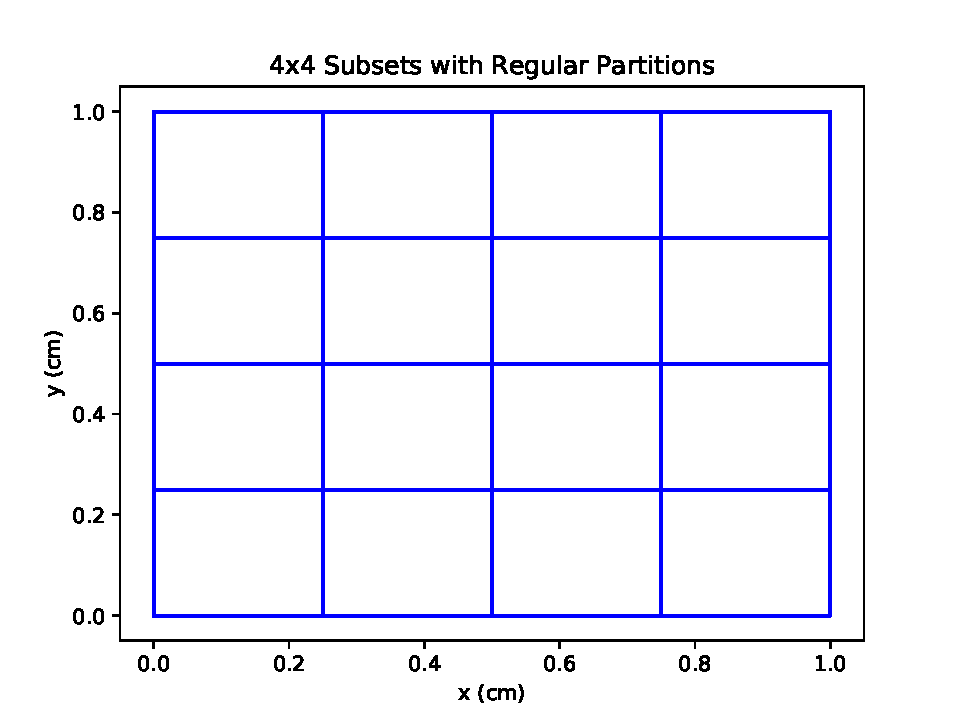
\includegraphics[scale=0.32]{../figures/cut_line_files/4_regular.pdf}
  \end{minipage}
  \begin{minipage}{0.49\textwidth}
    \centering
    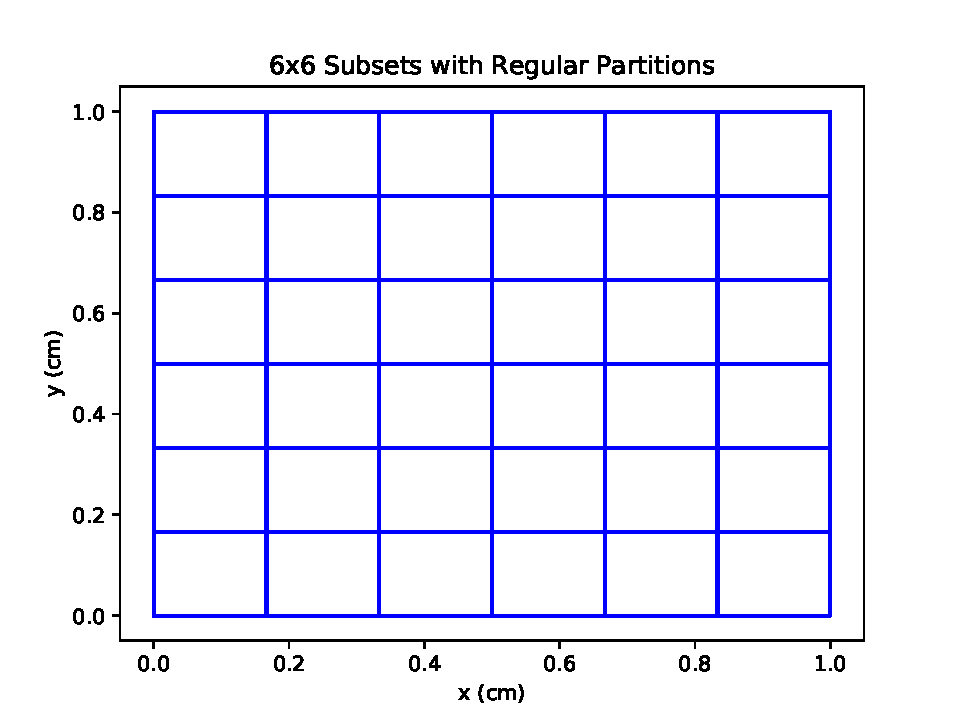
\includegraphics[scale=0.32]{../figures/cut_line_files/6_regular.pdf}
  \end{minipage}
  \begin{minipage}{0.49\textwidth}
    \centering
    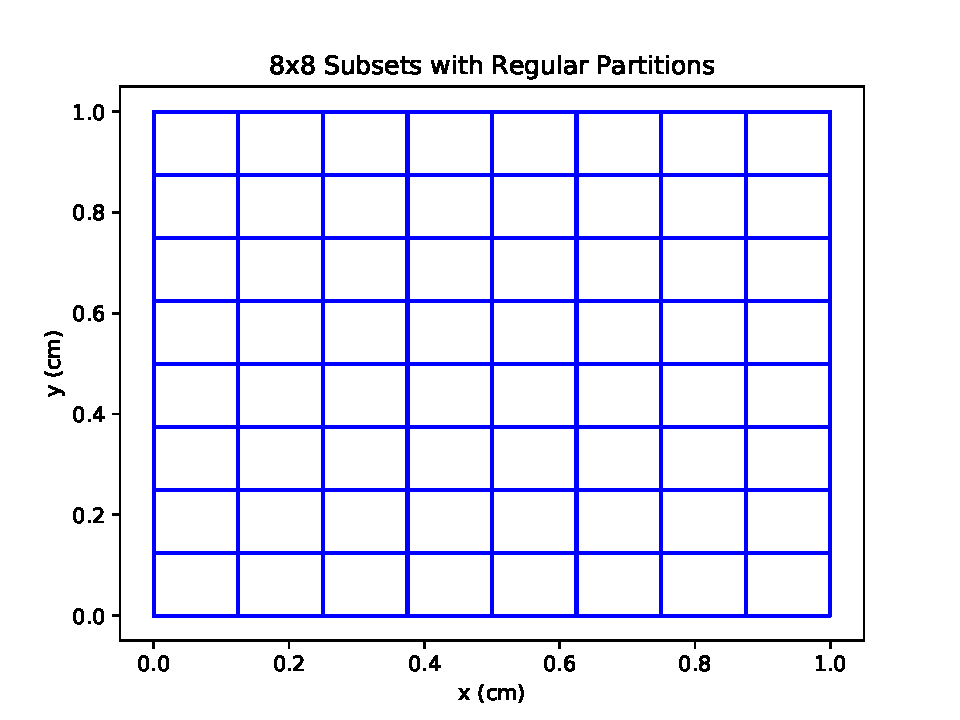
\includegraphics[scale=0.32]{../figures/cut_line_files/8_regular.pdf}
  \end{minipage}
  \begin{minipage}{0.49\textwidth}
    \centering
    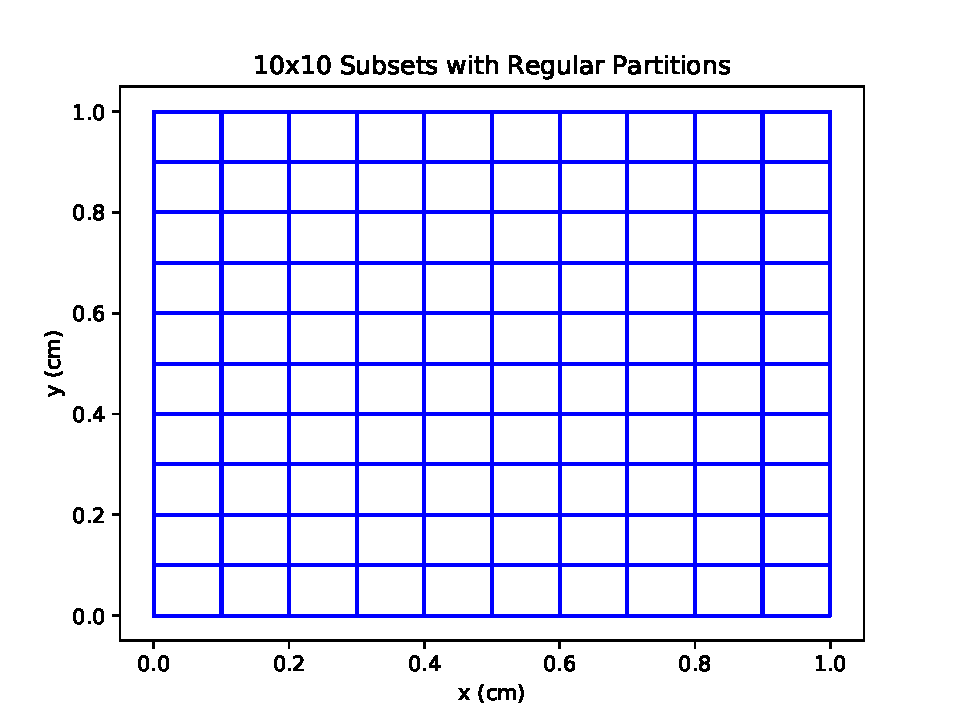
\includegraphics[scale=0.32]{../figures/cut_line_files/10_regular.pdf}
  \end{minipage}
\end{frame}

\begin{frame}[t]\frametitle{Regular Partitions}
  \centering
  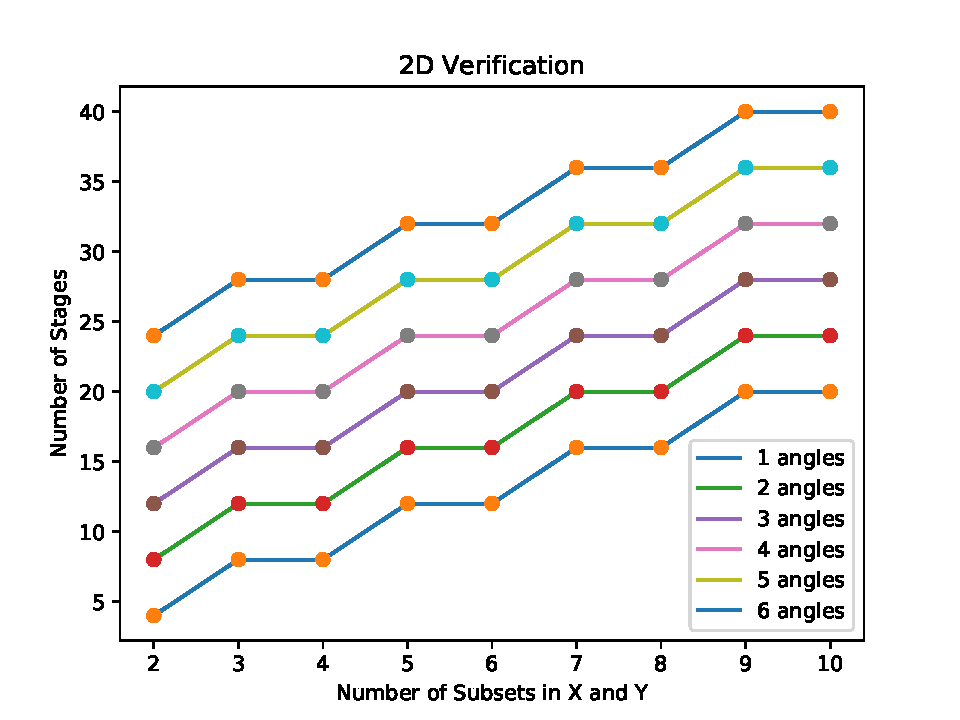
\includegraphics[scale=0.6]{../figures/regular_verification.pdf}
\end{frame}

\begin{frame}[t]\frametitle{``Mildly Random'' Partitions}
  \vspace{-.35cm}
   \begin{minipage}{0.49\textwidth}
    \centering
    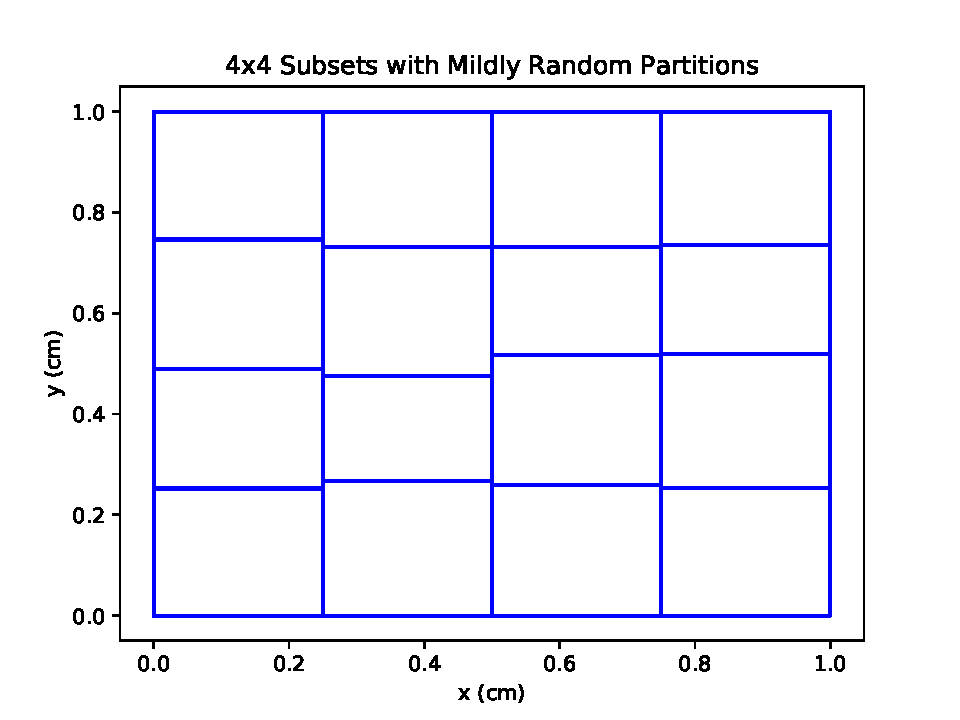
\includegraphics[scale=0.32]{../figures/cut_line_files/4_mild_random.pdf}
  \end{minipage}
  \begin{minipage}{0.49\textwidth}
    \centering
    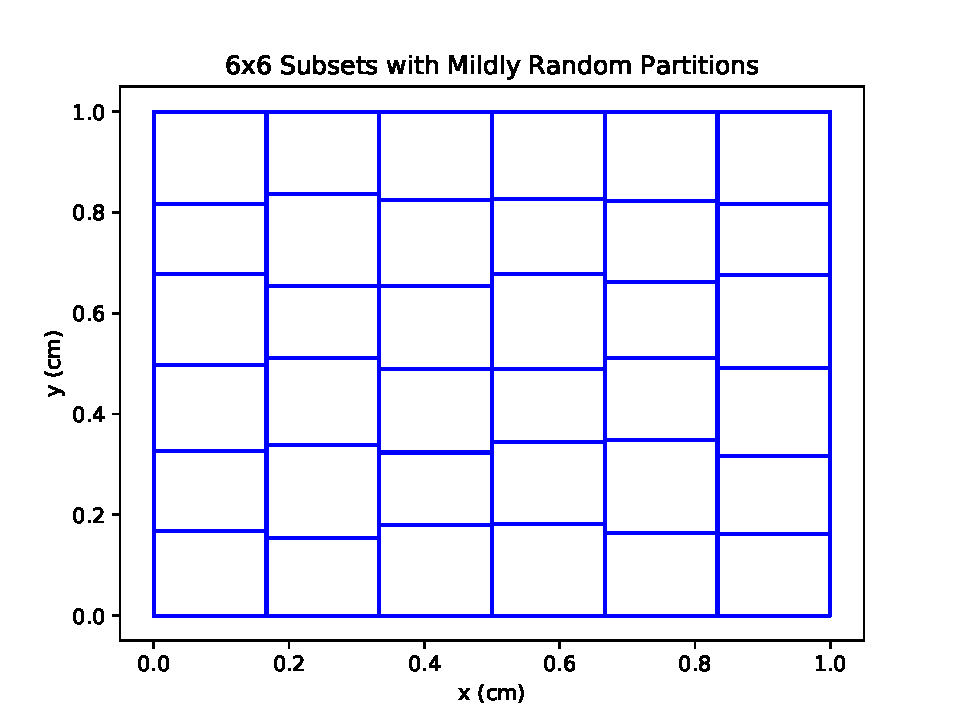
\includegraphics[scale=0.32]{../figures/cut_line_files/6_mild_random.pdf}
  \end{minipage}
  \begin{minipage}{0.49\textwidth}
    \centering
    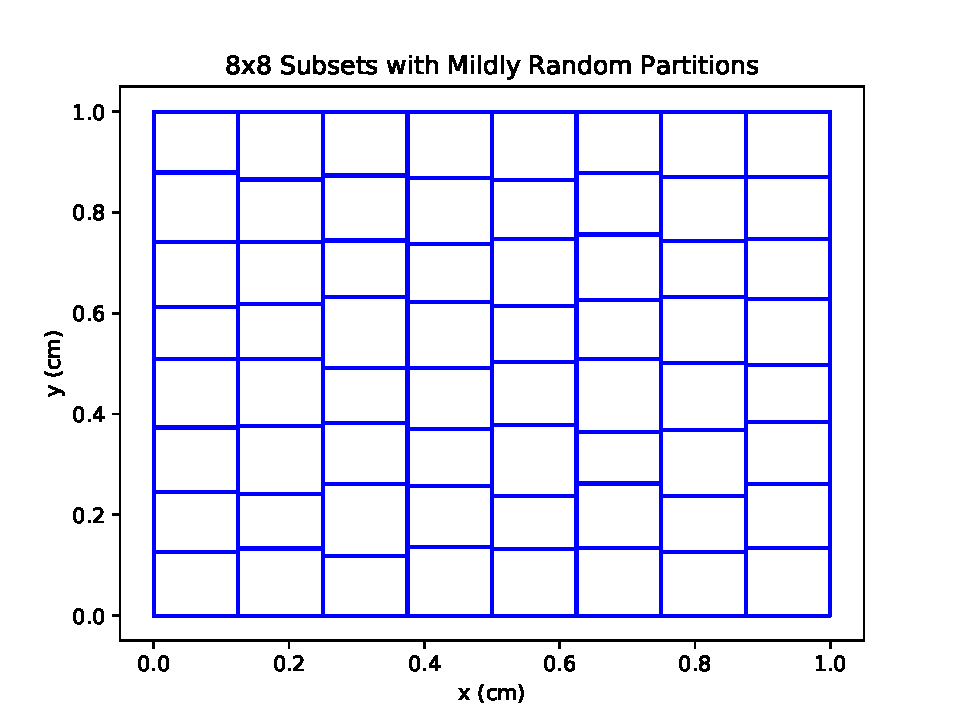
\includegraphics[scale=0.32]{../figures/cut_line_files/8_mild_random.pdf}
  \end{minipage}
  \begin{minipage}{0.49\textwidth}
    \centering
    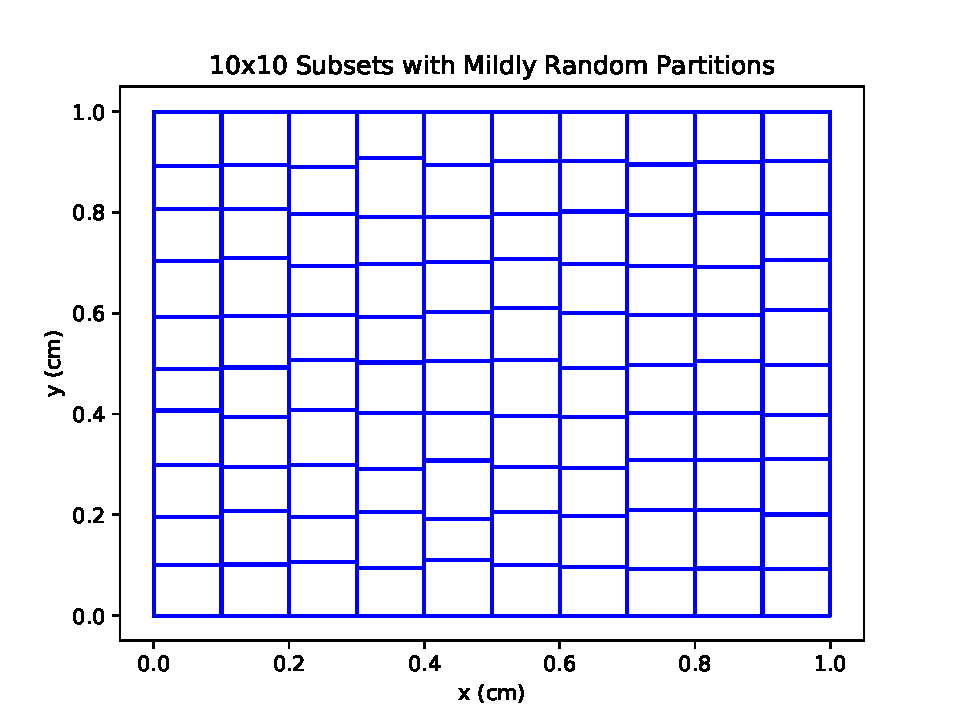
\includegraphics[scale=0.32]{../figures/cut_line_files/10_mild_random.pdf}
  \end{minipage}  
\end{frame}

\begin{frame}[t]\frametitle{``Mildly Random'' Partitions}
  \centering
  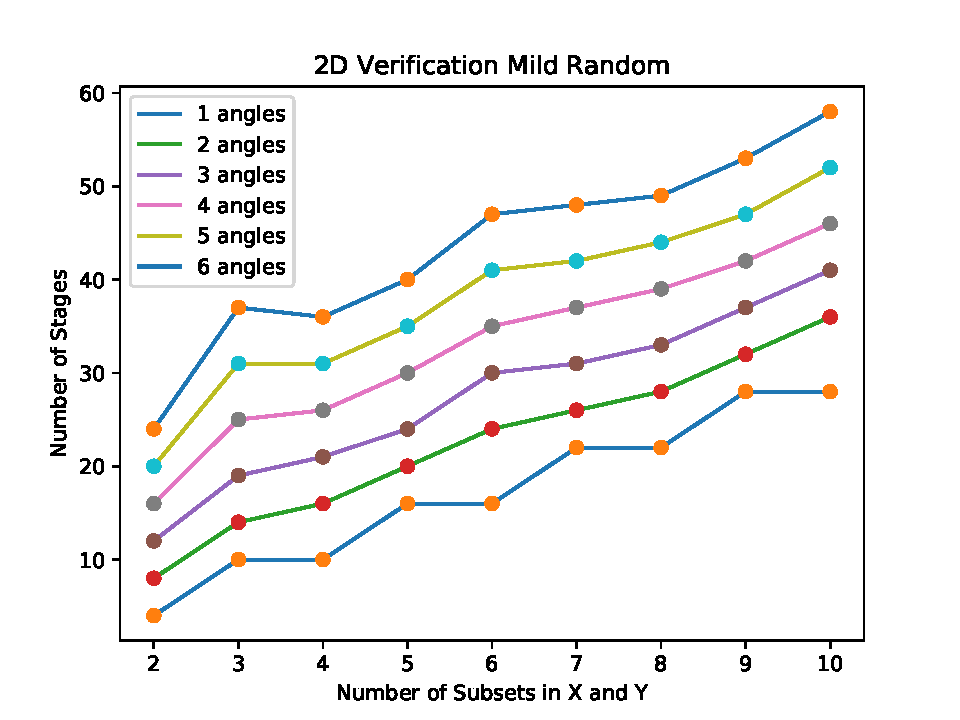
\includegraphics[scale=0.6]{../figures/mild_random_verification.pdf}
\end{frame}

\begin{frame}[t]\frametitle{``Random'' Partitions}
  \vspace{-.35cm}
   \begin{minipage}{0.49\textwidth}
    \centering
    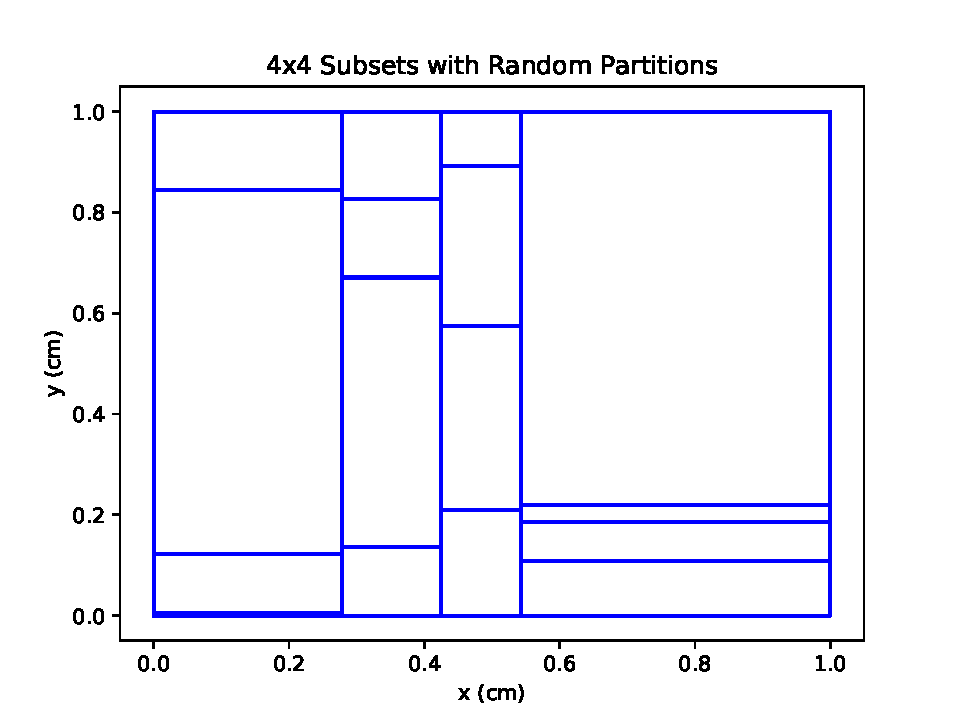
\includegraphics[scale=0.32]{../figures/cut_line_files/4_random.pdf}
  \end{minipage}
  \begin{minipage}{0.49\textwidth}
    \centering
    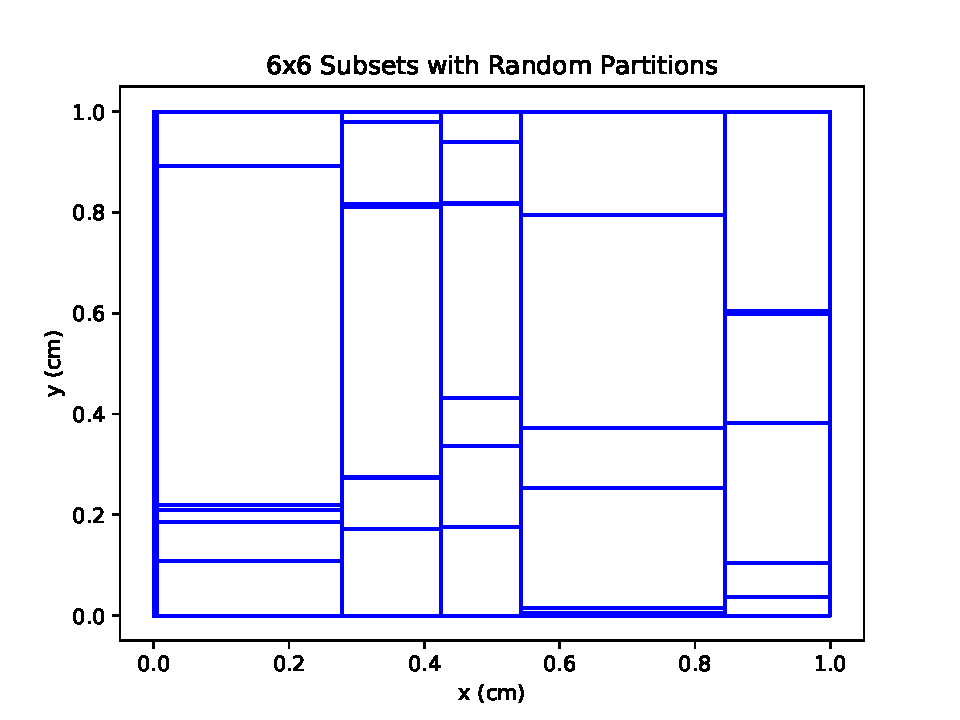
\includegraphics[scale=0.32]{../figures/cut_line_files/6_random.pdf}
  \end{minipage}
  \begin{minipage}{0.49\textwidth}
    \centering
    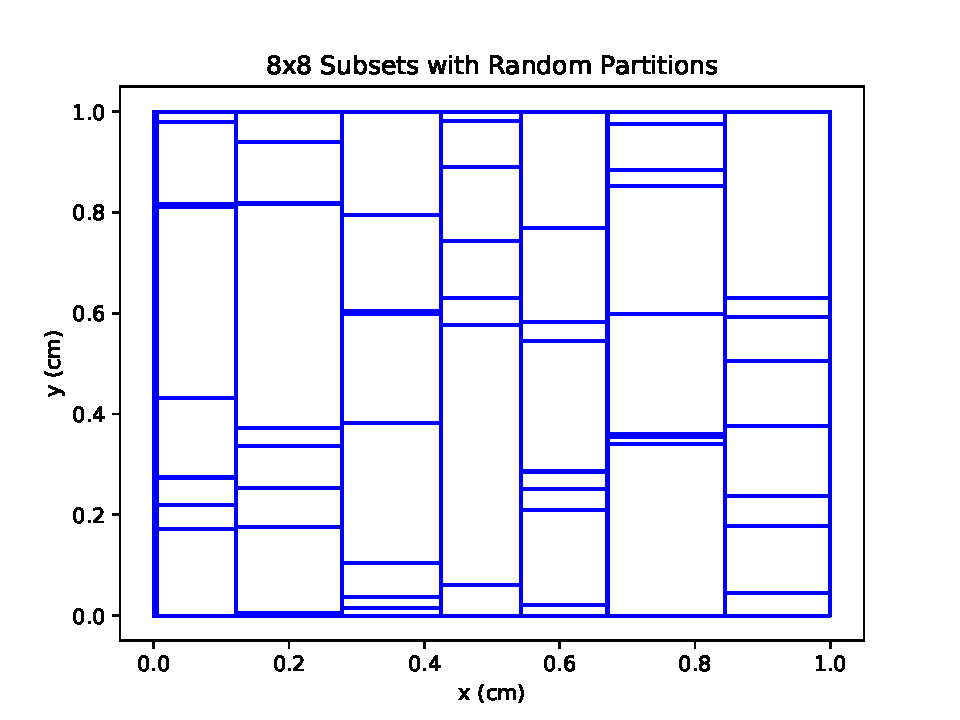
\includegraphics[scale=0.32]{../figures/cut_line_files/8_random.pdf}
  \end{minipage}
  \begin{minipage}{0.49\textwidth}
    \centering
    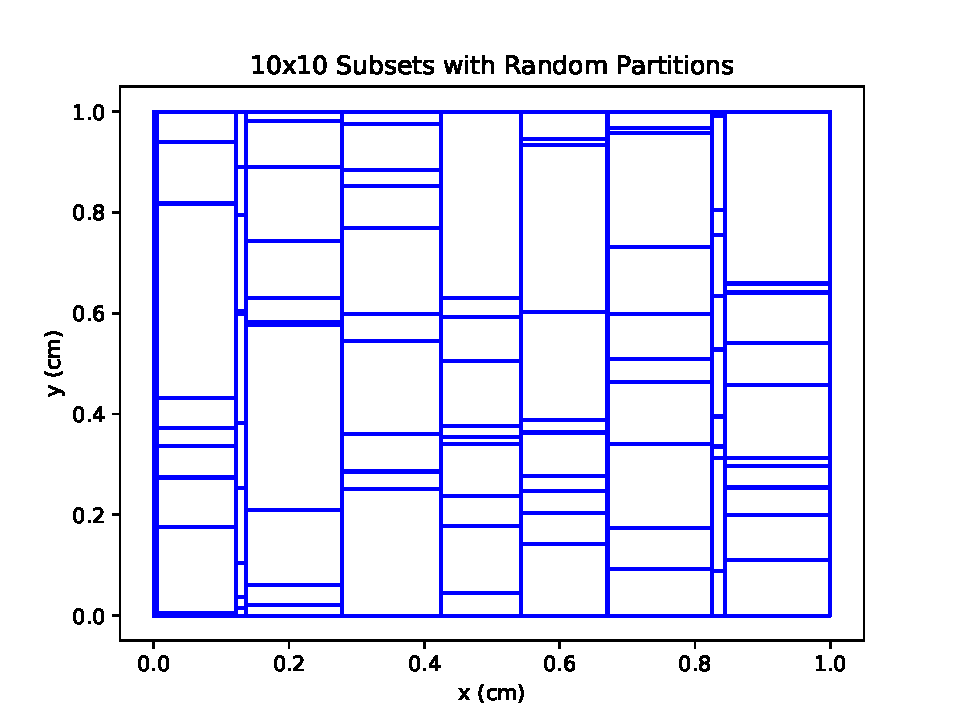
\includegraphics[scale=0.32]{../figures/cut_line_files/10_random.pdf}
  \end{minipage}  
\end{frame}

\begin{frame}[t]\frametitle{``Random'' Partitions}
  \centering
  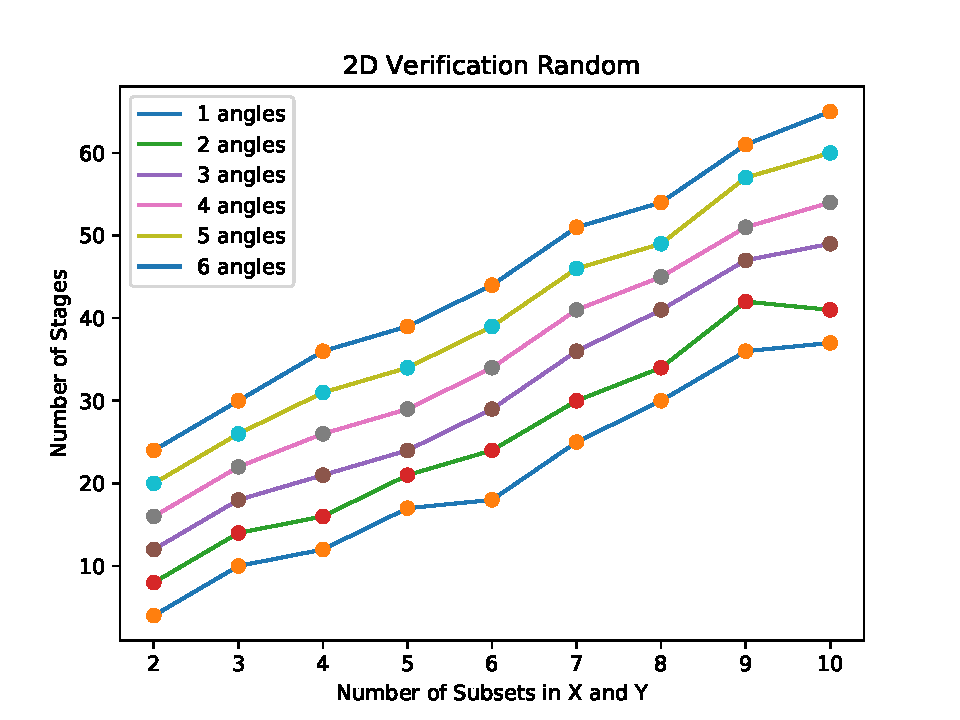
\includegraphics[scale=0.6]{../figures/random_verification.pdf}
\end{frame}

\begin{frame}[t]\frametitle{Probable Worst-Case Partitions}
  \vspace{-.35cm}
   \begin{minipage}{0.49\textwidth}
    \centering
    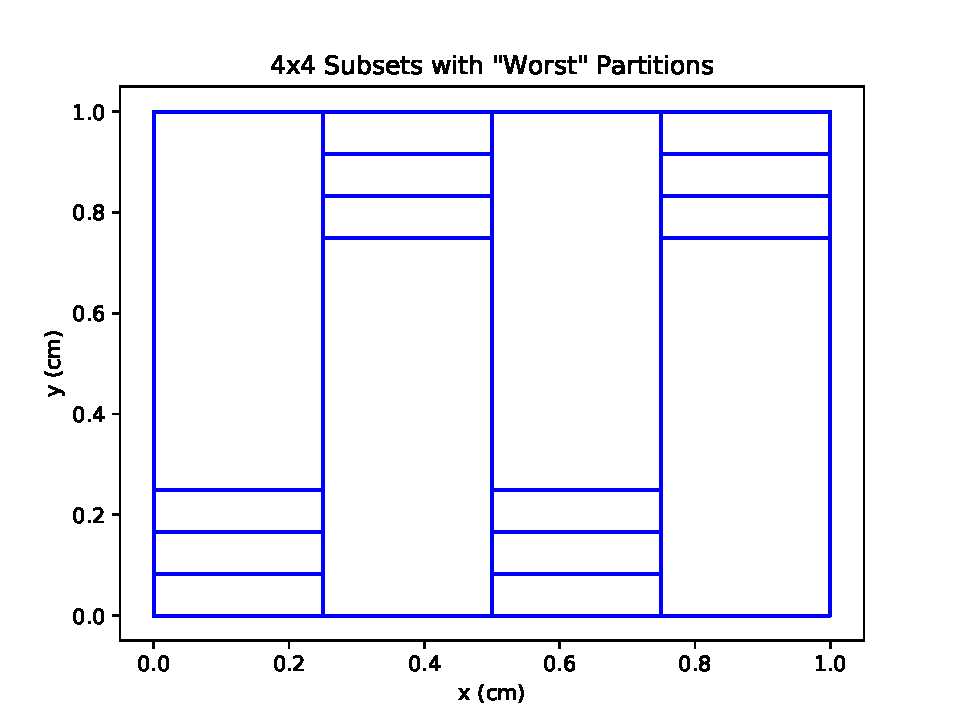
\includegraphics[scale=0.32]{../figures/cut_line_files/4_worst.pdf}
  \end{minipage}
  \begin{minipage}{0.49\textwidth}
    \centering
    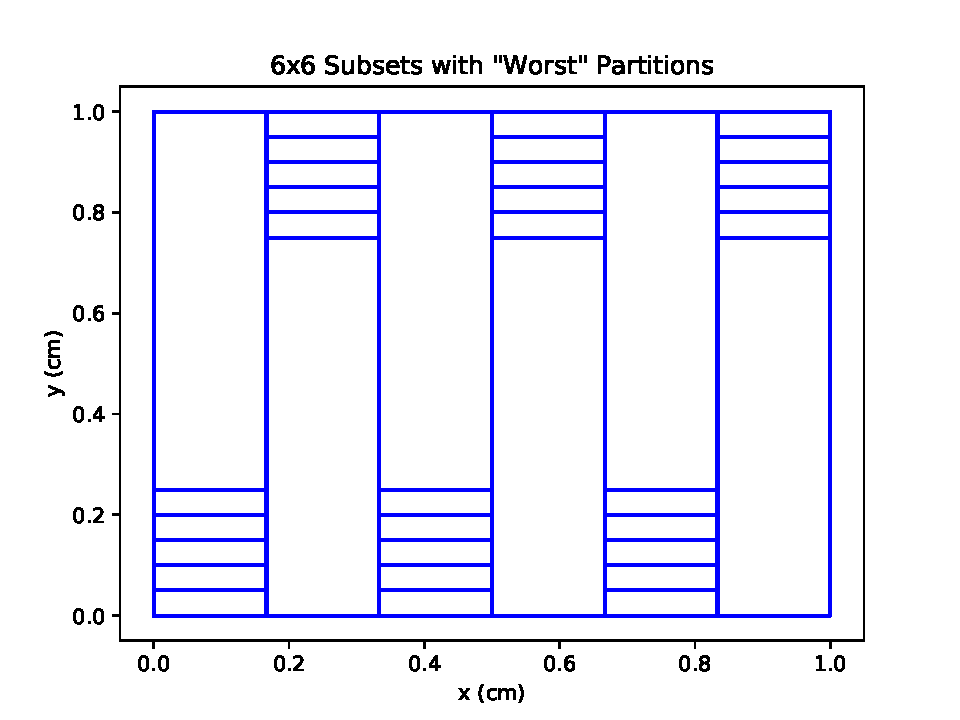
\includegraphics[scale=0.32]{../figures/cut_line_files/6_worst.pdf}
  \end{minipage}
  \begin{minipage}{0.49\textwidth}
    \centering
    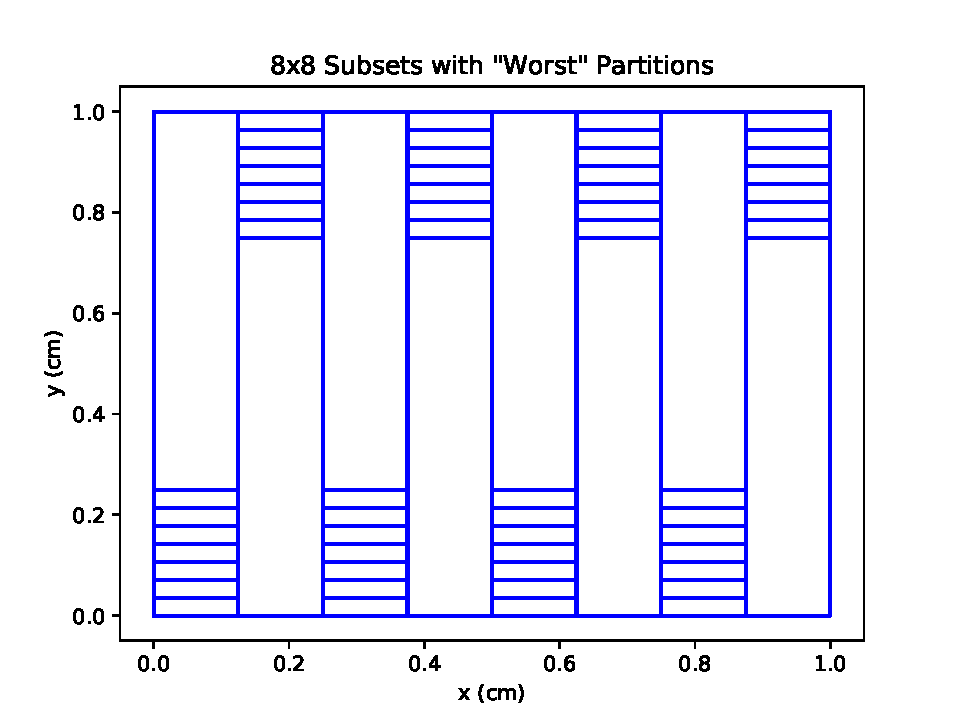
\includegraphics[scale=0.32]{../figures/cut_line_files/8_worst.pdf}
  \end{minipage}
  \begin{minipage}{0.49\textwidth}
    \centering
    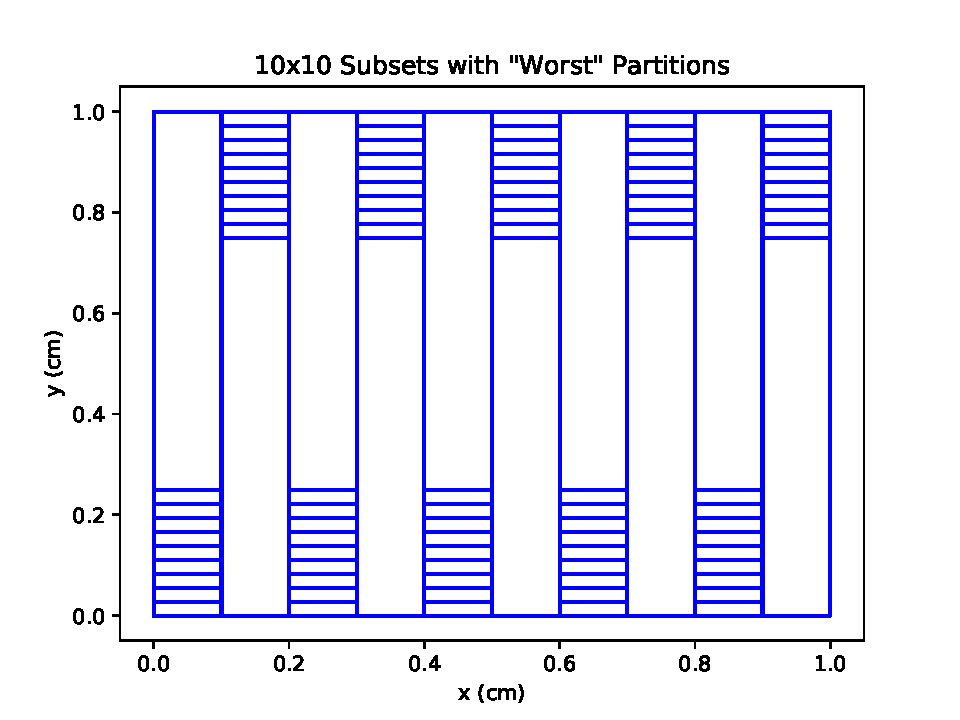
\includegraphics[scale=0.32]{../figures/cut_line_files/10_worst.pdf}
  \end{minipage}  
\end{frame}

\begin{frame}[t]\frametitle{Probable Worst-Case Partitions}
  \centering
  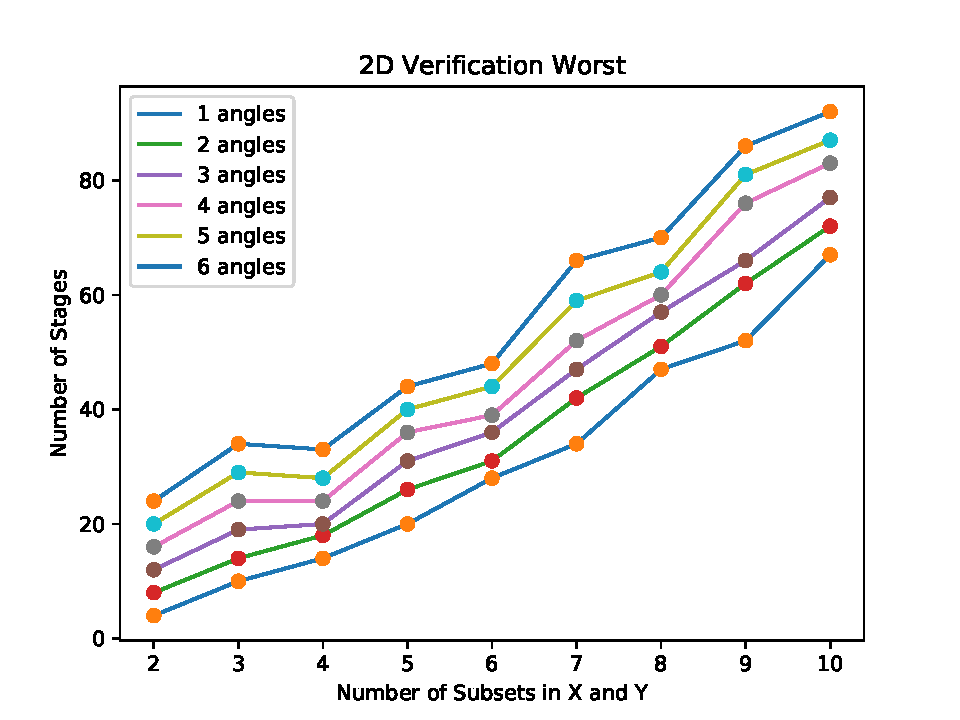
\includegraphics[scale=0.6]{../figures/worst_verification.pdf}
\end{frame}

\begin{frame}[t]\frametitle{3D Verification with Regular Partitions}
  \centering
  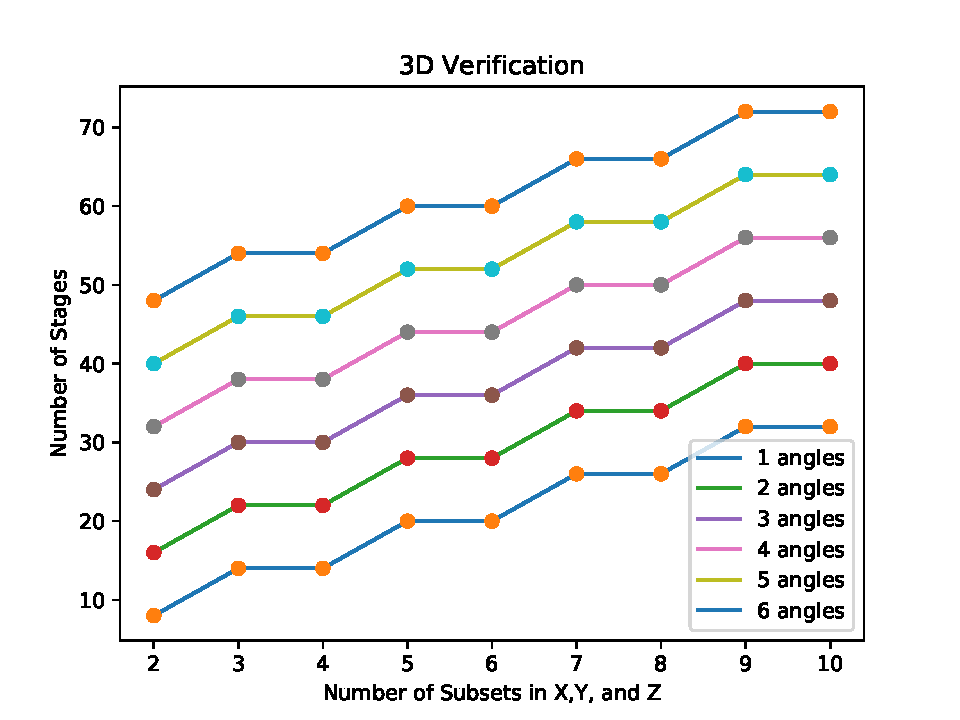
\includegraphics[scale=0.6]{../figures/3d_verification.pdf}
\end{frame}

\begin{frame}[t]\frametitle{Comparison to the 2018 Quartz Scaling Suite}
\begin{block}{}
  \begin{itemize}
    \item In 2018, PDT ran a scaling suite out to 90,112 cores on the Quartz supercomputer at LLNL.
    \item We ran the time-to-solution estimator for all cases out to 16,384 cores for comparison with PDT's and the performance model's time-per-sweep.
  \end{itemize}
\end{block}
\end{frame}

\begin{frame}[t]\frametitle{Stage count comparison to the 2018 Quartz scaling suite}
\centering
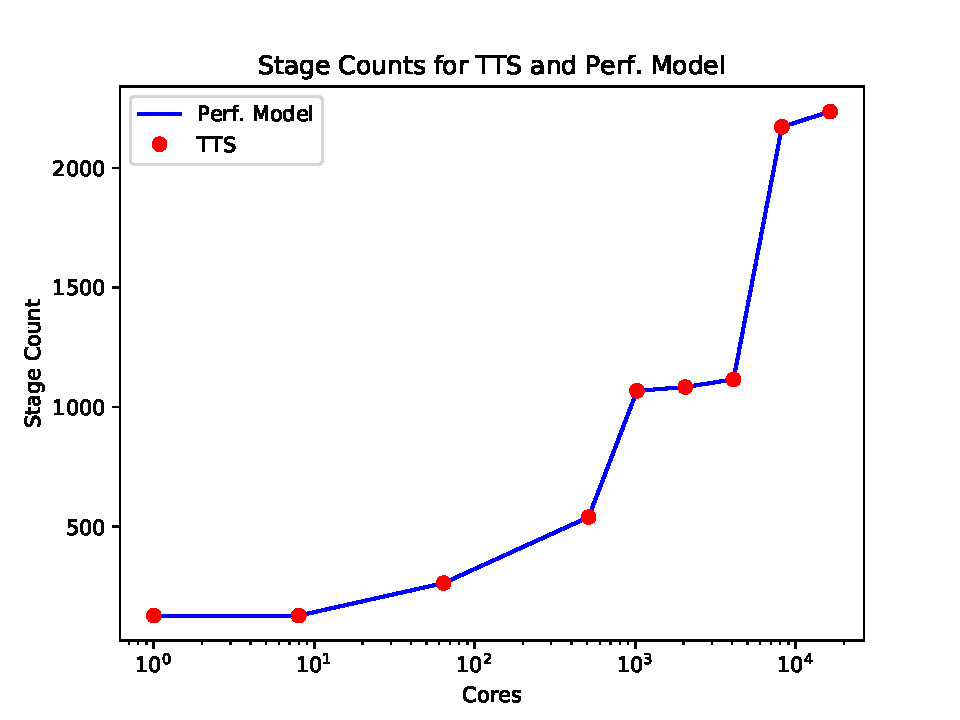
\includegraphics[scale=0.7]{../figures/scaling_stagecount.pdf}
\end{frame}

\begin{frame}[t]\frametitle{Sweep time comparison to the 2018 Quartz scaling suite}
\begin{minipage}[c]{0.5\textwidth}
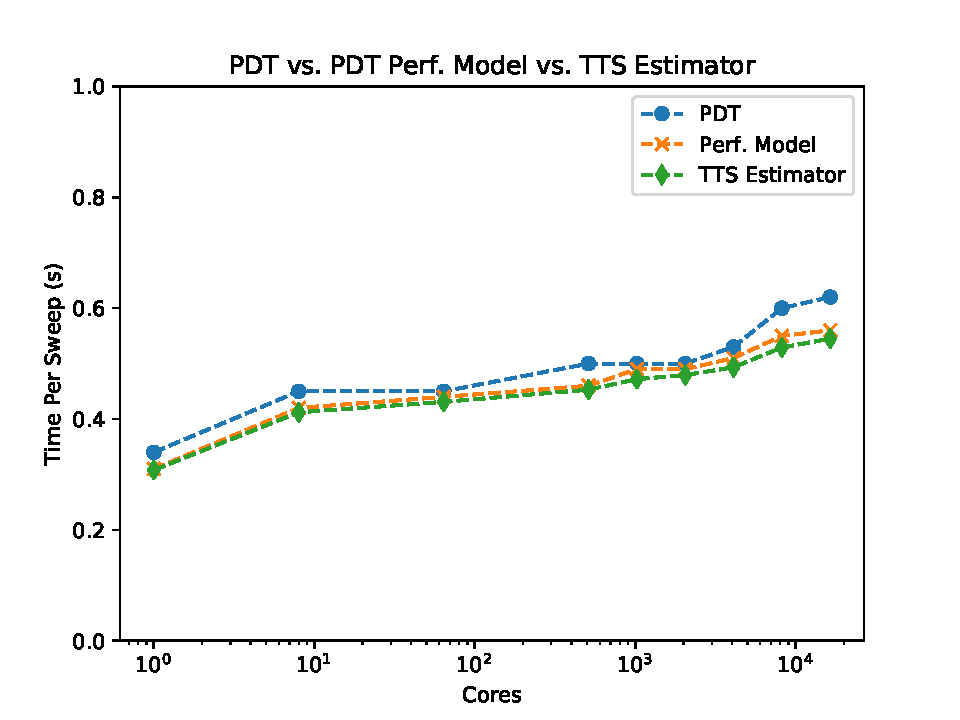
\includegraphics[scale=0.45]{../figures/scaling_tts_sweep_times.pdf}
\end{minipage}
\begin{minipage}[c]{0.48\textwidth}
\begin{table}[H]
\centering
\scalebox{0.75}{
\begin{tabular}{c|c|c|c}
\textbf{Cores} & \textbf{PDT v. Perf.} & \textbf{Perf. v. TTS} & \textbf{PDT v. TTS} \\ \hline
1&8.82\%&0.68\%&9.44\% \\ \hline
8&6.67\%&1.86\%&8.4\% \\ \hline
64&2.22\%&2.04\%&4.22\% \\ \hline
512&8.0\%&1.52\%&9.4\% \\ \hline
1024&2.0\%&3.67\%&5.6\% \\ \hline
2048&2.0\%&2.21\%&4.17\% \\ \hline
4096&3.77\%&3.24\%&6.89\% \\ \hline
8192&8.33\%&3.8\%&11.82\% \\ \hline
16384&9.68\%&2.7\%&12.11\%
\end{tabular}}
\end{table}
\end{minipage}
\begin{block}{}
\begin{itemize}
\item The PDT performance model is consistently higher than the performance model, in part due to the performance model assuming an equivalent cost per stage. 
\item In reality, not every processor communicates to 3 neighbors at every stage, and the final stage for each direction has no communication penalty. 
\end{itemize}
\end{block}
\end{frame}

\begin{frame}[t]\frametitle{Unbalanced Pin Comparison Between PDT and TTS}
  \centering
   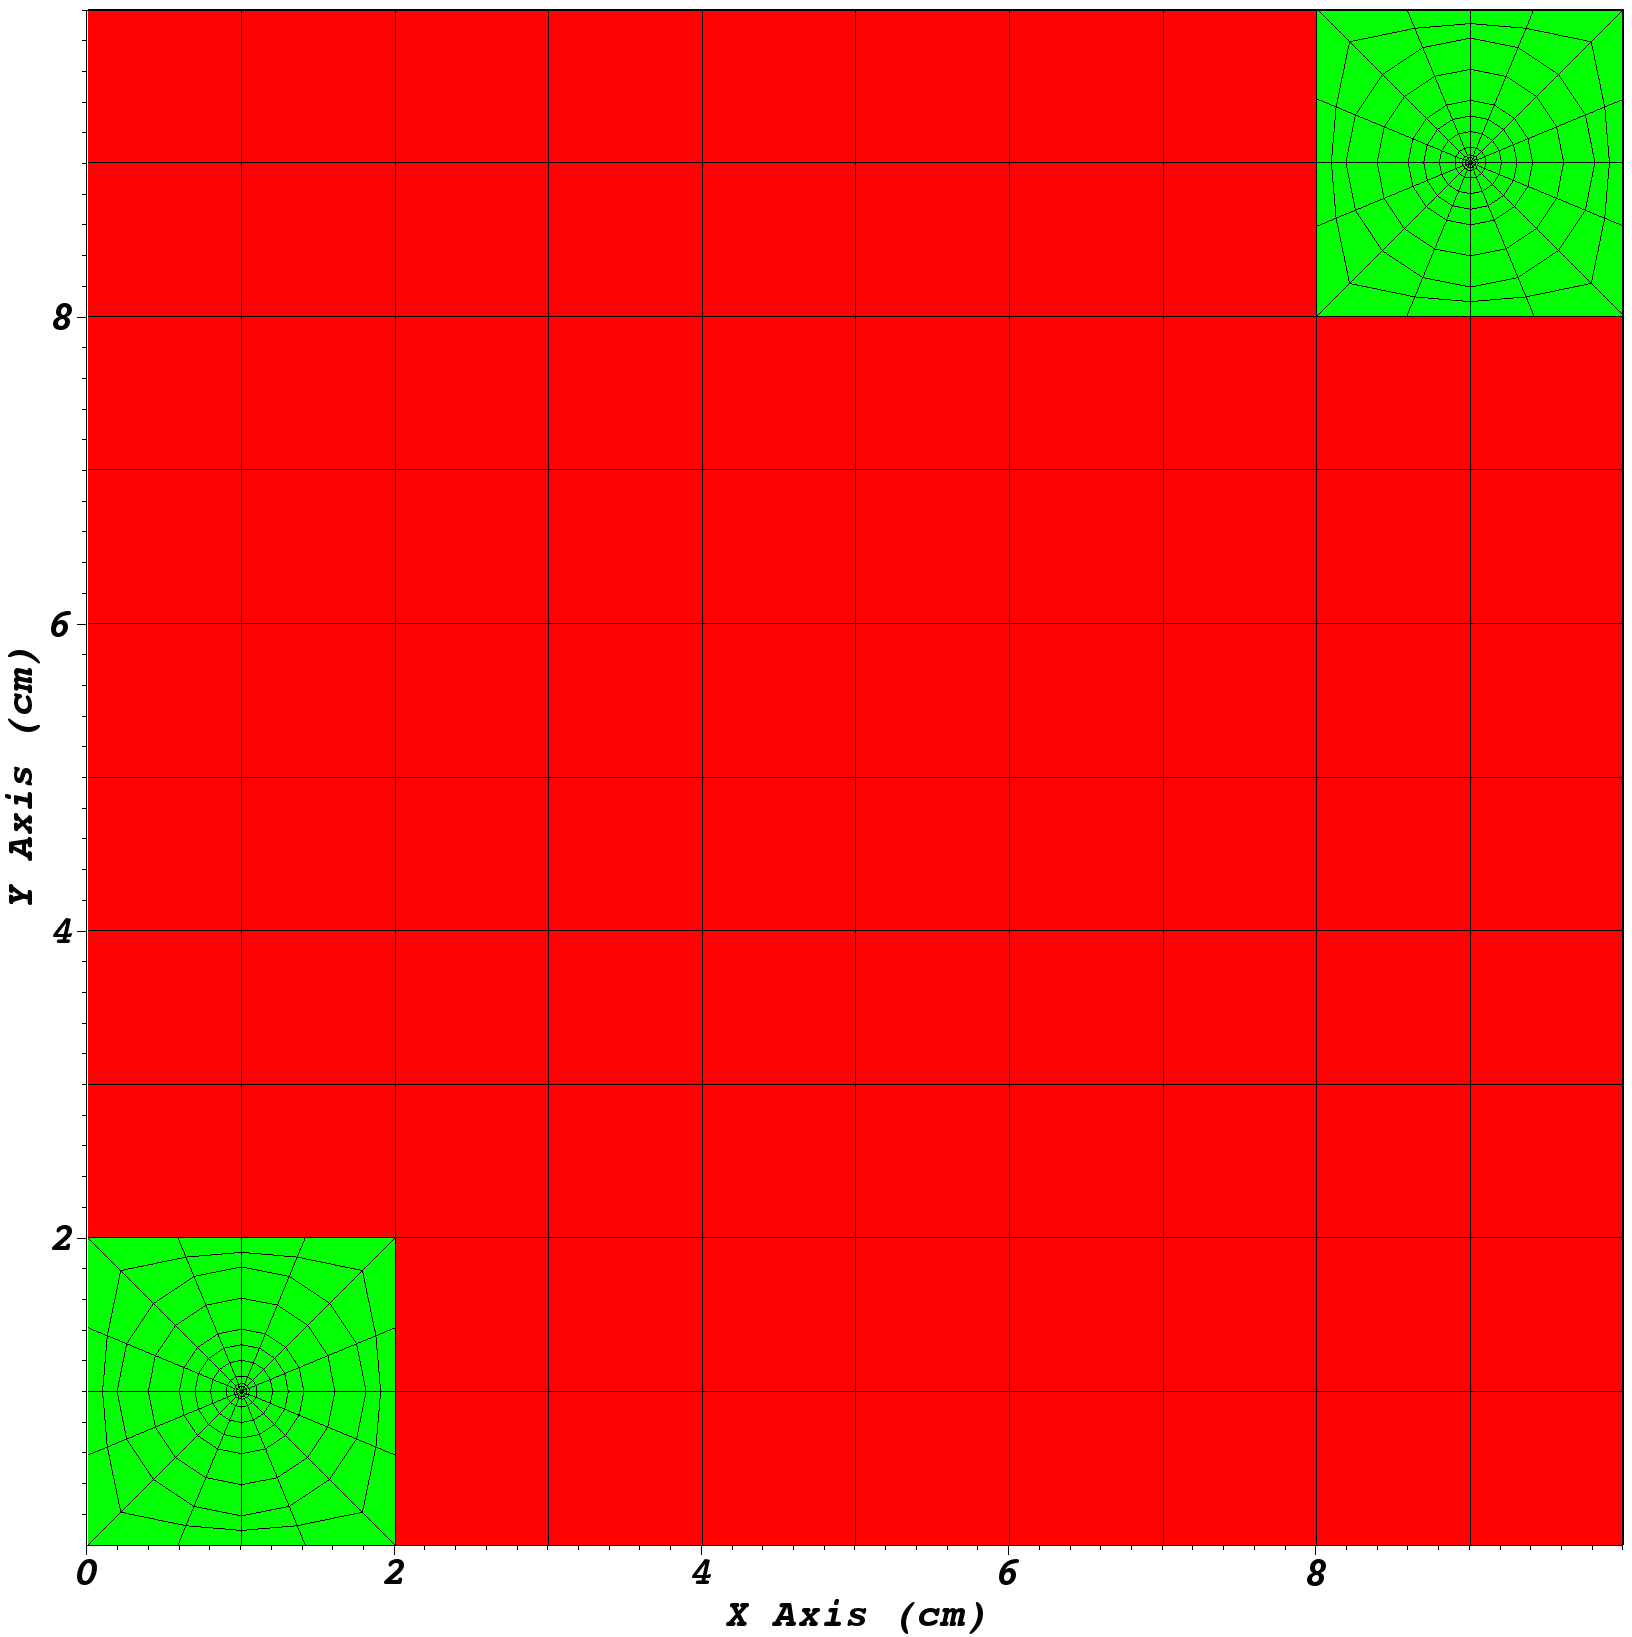
\includegraphics[scale=0.13]{../figures/spiderweb_10x10_sparse.png}
\end{frame}

\begin{frame}[t]\frametitle{Unbalanced Pin Comparison Between PDT and TTS}
\begin{block}{}
 Using the mesh from the previous slide, PDT and the time-to-solution estimator were run on the following problems:
 \begin{itemize}
   \item 2-10 subsets in each dimension with regular cuts.
   \item 2-10 subsets in each dimension with load-balanced cuts.
   \item 2-10 subsets in each dimension with load-balanced-by-dimension cuts.
 \end{itemize}
 Each case was run ten times in PDT, with ten transport sweeps each, to filter out outlying values.
\end{block}
\end{frame}

\begin{frame}[c]\frametitle{Unbalanced Pins with Regular Cuts}
\begin{minipage}[c]{0.5\textwidth}
\centering
\includegraphics[width=\textwidth]{../figures/spiderweb_reg_pdtvtts.pdf}
\end{minipage}
\begin{minipage}[c]{0.48\textwidth}
\centering
\begin{table}[H]
\centering
\begin{tabular}{c|c}
\textbf{$\sqrt{\text{Num Subsets}}$} & \bf PDT vs. TTS \\ \hline
2&19.93\%\\ \hline
3&12.3\%\\ \hline
4&1.75\%\\ \hline
5&15.69\%\\ \hline
6&2.71\%\\ \hline
7&2.61\%\\ \hline
8&4.45\%\\ \hline
9&3.21\%\\ \hline
10&11.38\%
\end{tabular}
\end{table}
\end{minipage}
\end{frame}

\begin{frame}[c]\frametitle{Unbalanced Pins with LB Cuts}
\begin{minipage}[c]{0.5\textwidth}
\centering
\includegraphics[width=\textwidth]{../figures/spiderweb_lb_pdtvtts.pdf}
\end{minipage}
\begin{minipage}[c]{0.48\textwidth}
\centering
\begin{table}[H]
\centering
\begin{tabular}{c|c}
\textbf{$\sqrt{\text{Num Subsets}}$} & \bf PDT vs. TTS \\ \hline
2&15.9\%\\ \hline
3&23.52\%\\ \hline
4&41.83\%\\ \hline
5&6.15\%\\ \hline
6&10.67\%\\ \hline
7&8.43\%\\ \hline
9&15.47\%\\ \hline
10&7.88\%
\end{tabular}
\end{table}

\end{minipage}
\end{frame}

\begin{frame}[c]\frametitle{Unbalanced Pins with LBD Cuts}
\begin{minipage}[c]{0.5\textwidth}
\centering
\includegraphics[width=\textwidth]{../figures/spiderweb_lbd_pdtvtts.pdf}
\end{minipage}
\begin{minipage}[c]{0.48\textwidth}
\centering
\begin{table}[!ht]
\centering
\begin{tabular}{c|c}
\textbf{$\sqrt{\text{Num Subsets}}$} & \bf PDT vs. TTS \\ \hline
2&6.5\%\\ \hline
3&13.49\%\\ \hline
4&4.04\%\\ \hline
6&2.78\%\\ \hline
7&3.5\%\\ \hline
9&4.18\%\\ \hline
10&12.01\%
\end{tabular}
\end{table}
\end{minipage}
\end{frame}

\begin{frame}[t]\frametitle{Conclusions drawn from the unbalanced pins suite}
\begin{block}{}
\begin{itemize}
  \item PDT's performance model agrees better the more unknowns there are.
  \item The unbalanced pin problem only contains 420 cells, which may explain why some of the larger discrepancies.
  \item PDT's first-come-first-serve scheduler is not always equivalent to the time-to-solution estimator's schedule, and is likelier to agree for LBD cases, where communication dependencies drive better agreement between the two schedules.
  \end{itemize}
\end{block}
\end{frame}

\begin{frame}[t]\frametitle{``Heavier'' unbalanced pin mesh with 9,656 cells}
\centering
\includegraphics[scale=0.14]{../figures/unbalanced_pins_more_sparse.png}
\end{frame}

\begin{frame}\frametitle{``Heavier unbalanced pin mesh with regular cuts}
\begin{minipage}[c]{0.5\textwidth}
\centering
\includegraphics[width=\textwidth]{../figures/more_sparse_reg_pdtvtts.pdf}
\end{minipage}
\begin{minipage}[c]{0.48\textwidth}
\centering
\begin{table}[H]
\centering
\begin{tabular}{c|c}
\textbf{$\sqrt{\text{Num Subsets}}$} & \bf PDT vs. TTS \\ \hline 
2&21.14\%\\ \hline 
3&15.87\%\\ \hline 
4&10.96\%\\ \hline 
5&9.3\%\\ \hline 
6&1.47\%\\ \hline 
7&0.41\%\\ \hline 
8&3.68\%\\ \hline 
9&2.85\%\\ \hline 
10&6.62\%
\end{tabular}
\end{table}
\end{minipage}
\begin{block}{}
With significantly more unknowns, we see better agreement numerically and in the trends of the two curves.
\end{block}
\end{frame}

\begin{frame}[c]\frametitle{The Level-2 experiment: 2,452 cells}
\centering
\includegraphics[scale=0.2]{../figures/level2_nocut.png}
\end{frame}

\begin{frame}[t]\frametitle{The Level-2 experiment partitioned into 42x13 subsets, regular and balanced}
\centering
\includegraphics[scale=0.15]{../figures/level2_42x13.png} \\
\centering
\includegraphics[scale=0.15]{../figures/level2_42x13_balanced.png}
\end{frame}

\begin{frame}[t]\frametitle{Level-2 experiment: PDT vs. TTS}
\begin{table}[ht]
\centering
\caption{The sweep times for the regular cut and balanced cut Level-2 problems for PDT and the time-to-solution estimator.}
\label{level2_sweep_times}
\begin{tabular}{c|c|c|c|c}
\bf Case & \bf PDT (s) & \bf TTS (s) & \bf PDT Min (s) & \bf PDT Max (s) \\ \hline
Regular & 0.07 & 0.0648 & 0.0686 & 0.0889\\ \hline
Balanced & 0.0531 & 0.0535 & 0.0522 & 0.0638
\end{tabular}
\end{table}
\begin{table}[ht]
\centering
\caption{The percent difference for the regular cut and balanced cut Level-2 problems between PDT and the time-to-solution estimator.}
\label{level2_percent_diff}
\begin{tabular}{c|c}
\textbf{Case} & \bf PDT vs. TTS \\ \hline
Regular & 7.52\% \\ \hline
Balanced & 0.63\%
\end{tabular}
\end{table}
\end{frame}
%%%%%%%%%%%%%%%%%%%%%%%%%%%%%%%%%%%%%%%%%%%%%%%%%%
\section{Partitioning Optimization}
\subsection{}
%%%%%%%%%%%%%%%%%%%%%%%%%%%%%%%%%%%%%%%%%%%%%%%%%%%
\begin{frame}[t]\frametitle{Choosing optimal partitions}
\begin{block}{}
  \begin{itemize}
    \item The time-to-solution estimator provides us with the time-to-solution given a set of partitioning parameters.
    \item The next step is to use the time-to-solution estimator to choose the optimal partitions.
    \item This was initially attempted using the scipy.optimize.minimize library but after extensive trials, tests, and research into ``black box'' methods, it became clear that the time-to-solution estimator function is not smooth enough to be used with bounded and constrained optimization methods.
    \item A method that is unique to our problem, which we have named the CDF method, was developed.
  \end{itemize}
\end{block}
\end{frame}

\begin{frame}[t]\frametitle{The CDF optimization method}
\begin{block}{}
\begin{itemize}
\item This method prioritizes cut line locations that minimizes the addition of cells to a mesh. 
\item We use the detailed vertex CDF to identify locations that coincide with ``natural boundaries'', or mesh boundaries that coincide with potential subset boundaries.
\item For a mesh, the method will:
\begin{enumerate}
  \item Find the most suitable natural boundaries in the $x$ dimension,
  \item For each set of columns, find the most suitable natural boundaries in the $y$ dimension,
  \item Run all iterations of cut lines selected.
  \item Run regular, load-balanced, load-balanced by dimension cuts.
  \item Select minimum time-to-solution.
\end{enumerate}
\end{itemize}
\end{block}
\end{frame}

\begin{frame}[t]\frametitle{Finding natural boundaries}
\begin{block}{}
Let's reconsider the unbalanced pin mesh, where there are natural boundaries at each centimeter in each dimension.
\end{block}
\centering
\includegraphics[scale=0.11]{../figures/spiderweb_10x10_sparse.png}
\end{frame}

\begin{frame}[t]\frametitle{The x-vertex CDF of the unbalanced pin mesh}
\centering
\includegraphics[scale=0.325]{../figures/xvertexcdf.pdf} \\
\includegraphics[scale=0.325]{../figures/gradcdf.pdf}
\end{frame}

\begin{frame}[t]\frametitle{Selection of cut lines}
\begin{block}{}
Once $x$ cut lines are selected, we choose $y$ cut lines for a series of column sets. \\
\begin{enumerate}
  \item Select highest $y$ jumps through all 4 columns of the mesh.
  \item Select the highest $y$ jumps through the first two columns, then the second two columns.
  \item Select the highest $y$ jumps for each column.
\end{enumerate}
\end{block}
\centering
\includegraphics[scale=0.4]{../figures/binary_tree.pdf}
\end{frame}

\section{Conclusions and Future Work}
\subsection{}

\begin{frame}[t]\frametitle{Lessons Learned comparing to PDT}
  \begin{block}{}
    \begin{itemize}
      \item Many of the PDT runs either crashed in the stitcher or hung once the sweep began (likely due to cycles). Some of these issues are expected to be resolved once Sweep Plane Data Structures are implemented in PDT.  
      \item All PDT problems were run on quartz at LLNL, an x86 machine. 
      \item The results from PDT runs were a bit noisy, which is the reason the median value of 10 runs were taken to weed out outliers. In the future, comparisons to PDT can be run on BGQ machine, which should be less noisy.
      \item Future work should include feeding the scheduler output from the time-to-solution estimator directly into PDT to get as accurate a comparison as possible (potentially a future Master's thesis?).
    \end{itemize}
  \end{block}
\end{frame}

\begin{frame}[t]\frametitle{Lessons Learned during Optimization}
  \begin{block}{}
    \begin{itemize}
    \item The \textbf{scipy.optimize.minimize} libraries are finding local minima, and the parameters are not traversing the entire boundaries before converging.
    \item Combining the local minimization method with a stochastic global minimization method yielded improved
      results, but still depended strongly on the initial parameter guess.
     \item The python optimization libraries do not consistently respect the parameter boundaries passed in. This causes the time-to-solution estimator to fail, and the optimizer to crash.
    \item The time-to-solution-estimator needs to be sped up significantly if larger cases are expected to run in reasonable amounts of time. The target is a few minutes for large cases, which currently can take up to a day, if they don't crash.  
    \end{itemize}
  \end{block}
\end{frame}

\begin{frame}[t]\frametitle{Future Work}
\begin{block}{Immediate Priorities}
  \begin{itemize}
    \item Speed up TTS! Problems modeling greater than 1000 subsets take about 1.5 mins to solve. 
    \item With the optimization tools evaluating the time-to-solution up to 10,000 times, this is extremely costly.
  \end{itemize}
\end{block}
\begin{block}{}
\begin{itemize}
  \item Explore a wider variety of optimization tools that can optimize large parameter spaces. 
  \item Potentially move to C++ in order to faster than python, and open up the possibility to better optimization tools.
  \end{itemize}
\end{block}

\end{frame}

\begin{frame}[t]\frametitle{Acknowledgements}
\begin{block}{}
A special thank you to the following individuals for their help and support:
\begin{itemize}
\item Drs. Ragusa, Morel, Adams, and Amato
\item Michael Adams, Daryl Hawkins, Timmie Smith
\item Andrew Till
\item The CERT team and fellow grad students (particularly my officemate Ian Halvic, who has dealt with my screaming). 
\end{itemize}
\end{block}
\end{frame}

\end{document}
